\documentclass[12pt,ngerman,]{book}
\usepackage{lmodern}
\usepackage{amssymb,amsmath}
\usepackage{ifxetex,ifluatex}
\usepackage{fixltx2e} % provides \textsubscript
\ifnum 0\ifxetex 1\fi\ifluatex 1\fi=0 % if pdftex
  \usepackage[T1]{fontenc}
  \usepackage[utf8]{inputenc}
\else % if luatex or xelatex
  \ifxetex
    \usepackage{mathspec}
  \else
    \usepackage{fontspec}
  \fi
  \defaultfontfeatures{Ligatures=TeX,Scale=MatchLowercase}
\fi
% use upquote if available, for straight quotes in verbatim environments
\IfFileExists{upquote.sty}{\usepackage{upquote}}{}
% use microtype if available
\IfFileExists{microtype.sty}{%
\usepackage{microtype}
\UseMicrotypeSet[protrusion]{basicmath} % disable protrusion for tt fonts
}{}
\usepackage[margin=1in]{geometry}
\usepackage{hyperref}
\PassOptionsToPackage{usenames,dvipsnames}{color} % color is loaded by hyperref
\hypersetup{unicode=true,
            pdftitle={Praxis der Datenanalyse},
            pdfauthor={Sebastian Sauer, Matthias Gehrke, Karsten Lübke, Oliver Gansser},
            colorlinks=true,
            linkcolor=Maroon,
            citecolor=Blue,
            urlcolor=Blue,
            breaklinks=true}
\urlstyle{same}  % don't use monospace font for urls
\ifnum 0\ifxetex 1\fi\ifluatex 1\fi=0 % if pdftex
  \usepackage[shorthands=off,main=ngerman]{babel}
\else
  \usepackage{polyglossia}
  \setmainlanguage[]{german}
\fi
\usepackage{color}
\usepackage{fancyvrb}
\newcommand{\VerbBar}{|}
\newcommand{\VERB}{\Verb[commandchars=\\\{\}]}
\DefineVerbatimEnvironment{Highlighting}{Verbatim}{commandchars=\\\{\}}
% Add ',fontsize=\small' for more characters per line
\usepackage{framed}
\definecolor{shadecolor}{RGB}{248,248,248}
\newenvironment{Shaded}{\begin{snugshade}}{\end{snugshade}}
\newcommand{\KeywordTok}[1]{\textcolor[rgb]{0.13,0.29,0.53}{\textbf{{#1}}}}
\newcommand{\DataTypeTok}[1]{\textcolor[rgb]{0.13,0.29,0.53}{{#1}}}
\newcommand{\DecValTok}[1]{\textcolor[rgb]{0.00,0.00,0.81}{{#1}}}
\newcommand{\BaseNTok}[1]{\textcolor[rgb]{0.00,0.00,0.81}{{#1}}}
\newcommand{\FloatTok}[1]{\textcolor[rgb]{0.00,0.00,0.81}{{#1}}}
\newcommand{\ConstantTok}[1]{\textcolor[rgb]{0.00,0.00,0.00}{{#1}}}
\newcommand{\CharTok}[1]{\textcolor[rgb]{0.31,0.60,0.02}{{#1}}}
\newcommand{\SpecialCharTok}[1]{\textcolor[rgb]{0.00,0.00,0.00}{{#1}}}
\newcommand{\StringTok}[1]{\textcolor[rgb]{0.31,0.60,0.02}{{#1}}}
\newcommand{\VerbatimStringTok}[1]{\textcolor[rgb]{0.31,0.60,0.02}{{#1}}}
\newcommand{\SpecialStringTok}[1]{\textcolor[rgb]{0.31,0.60,0.02}{{#1}}}
\newcommand{\ImportTok}[1]{{#1}}
\newcommand{\CommentTok}[1]{\textcolor[rgb]{0.56,0.35,0.01}{\textit{{#1}}}}
\newcommand{\DocumentationTok}[1]{\textcolor[rgb]{0.56,0.35,0.01}{\textbf{\textit{{#1}}}}}
\newcommand{\AnnotationTok}[1]{\textcolor[rgb]{0.56,0.35,0.01}{\textbf{\textit{{#1}}}}}
\newcommand{\CommentVarTok}[1]{\textcolor[rgb]{0.56,0.35,0.01}{\textbf{\textit{{#1}}}}}
\newcommand{\OtherTok}[1]{\textcolor[rgb]{0.56,0.35,0.01}{{#1}}}
\newcommand{\FunctionTok}[1]{\textcolor[rgb]{0.00,0.00,0.00}{{#1}}}
\newcommand{\VariableTok}[1]{\textcolor[rgb]{0.00,0.00,0.00}{{#1}}}
\newcommand{\ControlFlowTok}[1]{\textcolor[rgb]{0.13,0.29,0.53}{\textbf{{#1}}}}
\newcommand{\OperatorTok}[1]{\textcolor[rgb]{0.81,0.36,0.00}{\textbf{{#1}}}}
\newcommand{\BuiltInTok}[1]{{#1}}
\newcommand{\ExtensionTok}[1]{{#1}}
\newcommand{\PreprocessorTok}[1]{\textcolor[rgb]{0.56,0.35,0.01}{\textit{{#1}}}}
\newcommand{\AttributeTok}[1]{\textcolor[rgb]{0.77,0.63,0.00}{{#1}}}
\newcommand{\RegionMarkerTok}[1]{{#1}}
\newcommand{\InformationTok}[1]{\textcolor[rgb]{0.56,0.35,0.01}{\textbf{\textit{{#1}}}}}
\newcommand{\WarningTok}[1]{\textcolor[rgb]{0.56,0.35,0.01}{\textbf{\textit{{#1}}}}}
\newcommand{\AlertTok}[1]{\textcolor[rgb]{0.94,0.16,0.16}{{#1}}}
\newcommand{\ErrorTok}[1]{\textcolor[rgb]{0.64,0.00,0.00}{\textbf{{#1}}}}
\newcommand{\NormalTok}[1]{{#1}}
\usepackage{longtable,booktabs}
\usepackage{graphicx,grffile}
\makeatletter
\def\maxwidth{\ifdim\Gin@nat@width>\linewidth\linewidth\else\Gin@nat@width\fi}
\def\maxheight{\ifdim\Gin@nat@height>\textheight\textheight\else\Gin@nat@height\fi}
\makeatother
% Scale images if necessary, so that they will not overflow the page
% margins by default, and it is still possible to overwrite the defaults
% using explicit options in \includegraphics[width, height, ...]{}
\setkeys{Gin}{width=\maxwidth,height=\maxheight,keepaspectratio}
\IfFileExists{parskip.sty}{%
\usepackage{parskip}
}{% else
\setlength{\parindent}{0pt}
\setlength{\parskip}{6pt plus 2pt minus 1pt}
}
\setlength{\emergencystretch}{3em}  % prevent overfull lines
\providecommand{\tightlist}{%
  \setlength{\itemsep}{0pt}\setlength{\parskip}{0pt}}
\setcounter{secnumdepth}{5}
% Redefines (sub)paragraphs to behave more like sections
\ifx\paragraph\undefined\else
\let\oldparagraph\paragraph
\renewcommand{\paragraph}[1]{\oldparagraph{#1}\mbox{}}
\fi
\ifx\subparagraph\undefined\else
\let\oldsubparagraph\subparagraph
\renewcommand{\subparagraph}[1]{\oldsubparagraph{#1}\mbox{}}
\fi

%%% Use protect on footnotes to avoid problems with footnotes in titles
\let\rmarkdownfootnote\footnote%
\def\footnote{\protect\rmarkdownfootnote}

%%% Change title format to be more compact
\usepackage{titling}

% Create subtitle command for use in maketitle
\newcommand{\subtitle}[1]{
  \posttitle{
    \begin{center}\large#1\end{center}
    }
}

\setlength{\droptitle}{-2em}
  \title{Praxis der Datenanalyse}
  \pretitle{\vspace{\droptitle}\centering\huge}
  \posttitle{\par}
\subtitle{Skript zum Modul}
  \author{Sebastian Sauer, Matthias Gehrke, Karsten Lübke, Oliver Gansser}
  \preauthor{\centering\large\emph}
  \postauthor{\par}
  \predate{\centering\large\emph}
  \postdate{\par}
  \date{22 April, 2017}

\usepackage{booktabs}
\usepackage{longtable}
\usepackage[bf,singlelinecheck=off]{caption}

%\setmainfont[UprightFeatures={SmallCapsFont=AlegreyaSC-Regular}]{Alegreya}

\usepackage{framed,color}
\definecolor{shadecolor}{RGB}{248,248,248}

\renewcommand{\textfraction}{0.05}
\renewcommand{\topfraction}{0.8}
\renewcommand{\bottomfraction}{0.8}
\renewcommand{\floatpagefraction}{0.75}

%\renewenvironment{quote}{\begin{VF}}{\end{VF}}
\let\oldhref\href
\renewcommand{\href}[2]{#2\footnote{\url{#1}}}

\ifxetex
  \usepackage{letltxmacro}
  \setlength{\XeTeXLinkMargin}{1pt}
  \LetLtxMacro\SavedIncludeGraphics\includegraphics
  \def\includegraphics#1#{% #1 catches optional stuff (star/opt. arg.)
    \IncludeGraphicsAux{#1}%
  }%
  \newcommand*{\IncludeGraphicsAux}[2]{%
    \XeTeXLinkBox{%
      \SavedIncludeGraphics#1{#2}%
    }%
  }%
\fi

\renewcommand{\thesection}{\arabic{section}}  % ses




\makeatletter
\newenvironment{kframe}{%
\medskip{}
\setlength{\fboxsep}{.8em}
 \def\at@end@of@kframe{}%
 \ifinner\ifhmode%
  \def\at@end@of@kframe{\end{minipage}}%
  \begin{minipage}{\columnwidth}%
 \fi\fi%
 \def\FrameCommand##1{\hskip\@totalleftmargin \hskip-\fboxsep
 \colorbox{shadecolor}{##1}\hskip-\fboxsep
     % There is no \\@totalrightmargin, so:
     \hskip-\linewidth \hskip-\@totalleftmargin \hskip\columnwidth}%
 \MakeFramed {\advance\hsize-\width
   \@totalleftmargin\z@ \linewidth\hsize
   \@setminipage}}%
 {\par\unskip\endMakeFramed%
 \at@end@of@kframe}
\makeatother

\renewenvironment{Shaded}{\begin{kframe}}{\end{kframe}}

\newenvironment{rmdblock}[1]
  {
  \begin{itemize}
  \renewcommand{\labelitemi}{
    \raisebox{-.7\height}[0pt][0pt]{
      {\setkeys{Gin}{width=3em,keepaspectratio}\includegraphics{images/#1}}
    }
  }
  \setlength{\fboxsep}{1em}
  \begin{kframe}
  \item
  }
  {
  \end{kframe}
  \end{itemize}
  }
\newenvironment{rmdnote}
  {\begin{rmdblock}{note}}
  {\end{rmdblock}}
\newenvironment{rmdcaution}
  {\begin{rmdblock}{caution}}
  {\end{rmdblock}}
\newenvironment{rmdimportant}
  {\begin{rmdblock}{important}}
  {\end{rmdblock}}
\newenvironment{rmdtip}
  {\begin{rmdblock}{tip}}
  {\end{rmdblock}}
\newenvironment{rmdwarning}
  {\begin{rmdblock}{warning}}
  {\end{rmdblock}}
\newenvironment{rmdpseudocode}
  {\begin{rmdblock}{pseudocode}}
  {\end{rmdblock}}
\newenvironment{rmdexercises}
  {\begin{rmdblock}{exercises}}
  {\end{rmdblock}}
\newenvironment{rmdlove}
  {\begin{rmdblock}{love}}
  {\end{rmdblock}}

\usepackage{makeidx}
\makeindex

\urlstyle{tt}

\usepackage{amsthm}
\makeatletter
\def\thm@space@setup{%
  \thm@preskip=8pt plus 2pt minus 4pt
  \thm@postskip=\thm@preskip
}
\makeatother

\frontmatter

\let\BeginKnitrBlock\begin \let\EndKnitrBlock\end
\begin{document}
\maketitle

{
\hypersetup{linkcolor=black}
\setcounter{tocdepth}{2}
\tableofcontents
}
\listoftables
\listoffigures
\section*{Vorwort}\label{vorwort}


\section{Organisatorisches}\label{organisatorisches}

\section{Rahmen}\label{rahmen}

\section{Datenjudo}\label{datenjudo}

\BeginKnitrBlock{rmdcaution}
Lernziele:

\begin{itemize}
\tightlist
\item
  Typische Probleme der Datenanalyse schildern können.
\item
  Zentrale \texttt{dplyr}-Befehle anwenden können.
\item
  \texttt{dplyr}-Befehle kombinieren können.
\item
  Die Pfeife anwenden können.
\item
  Werte umkodieren und ``binnen'' können.
\end{itemize}
\EndKnitrBlock{rmdcaution}

\begin{figure}

{\centering 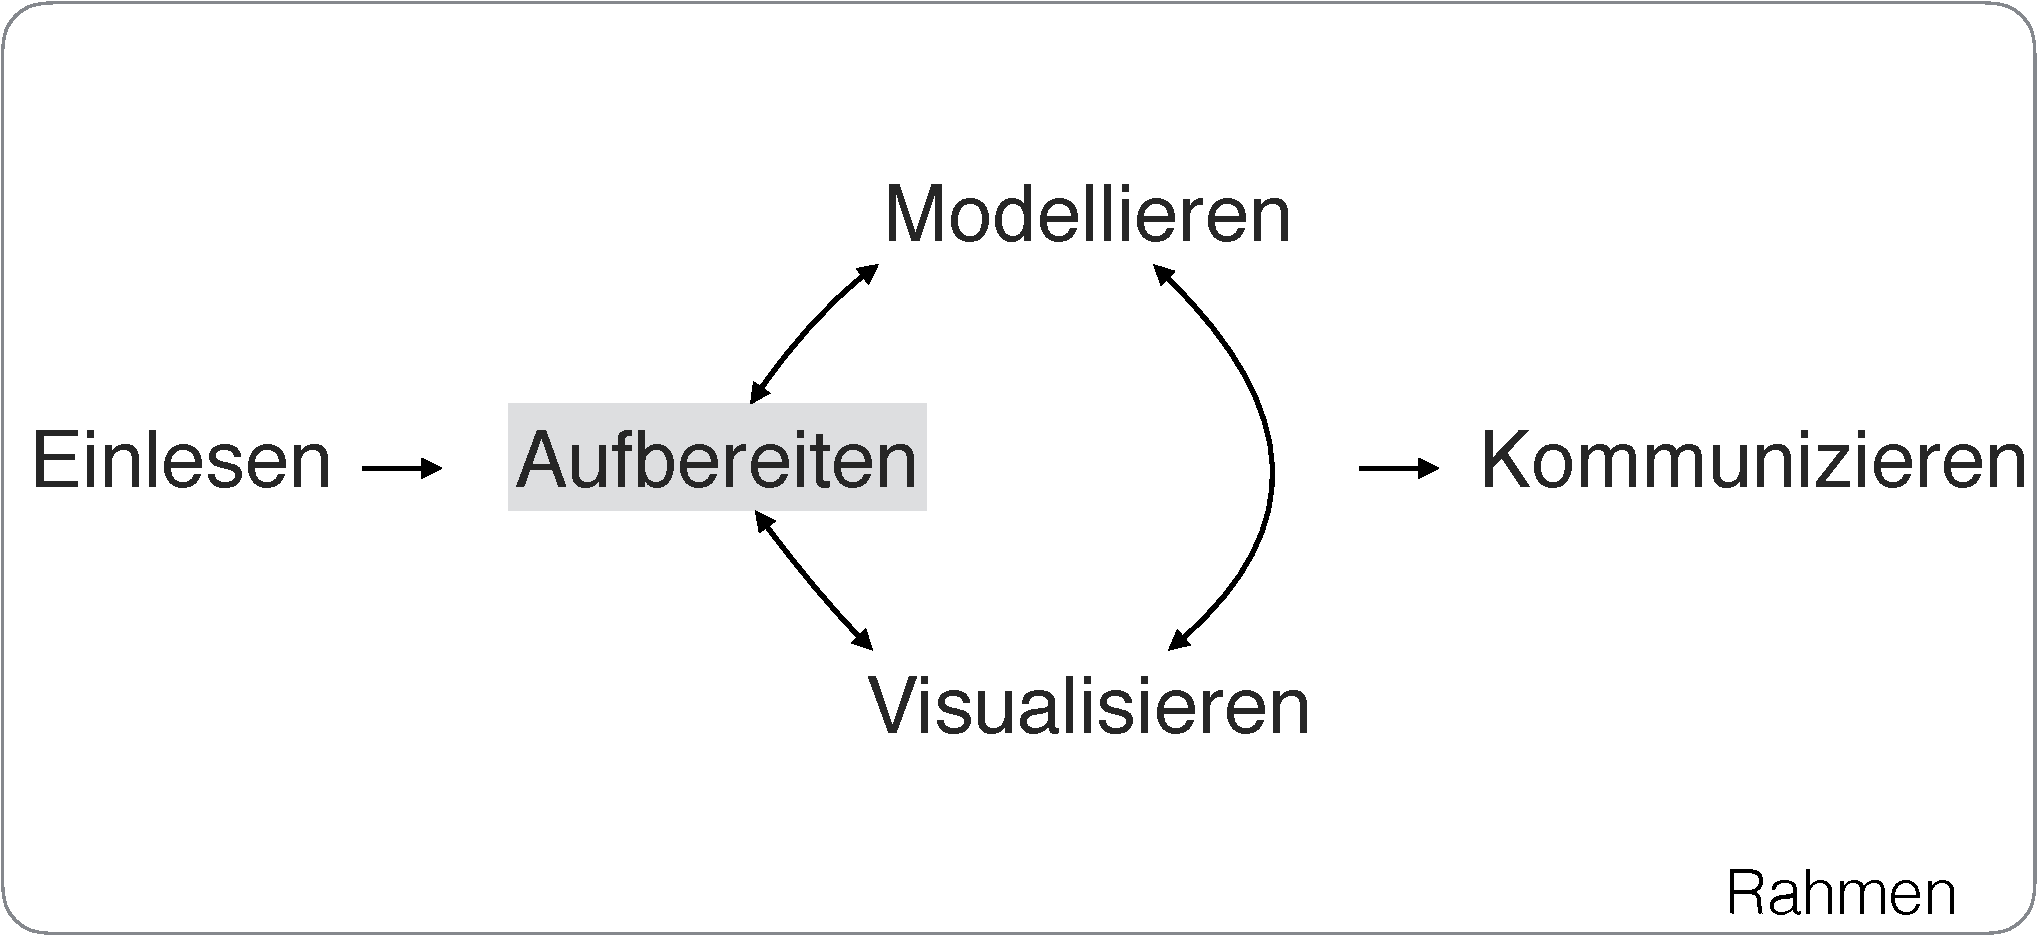
\includegraphics[width=0.7\linewidth]{images/Datenjudo/Aufbereiten} 

}

\caption{Daten aufbereiten}\label{fig:fig-datenjudo}
\end{figure}

In diesem Kapitel benötigte Pakete:

\begin{Shaded}
\begin{Highlighting}[]
\KeywordTok{library}\NormalTok{(tidyverse)  }\CommentTok{# Datenjudo}
\KeywordTok{library}\NormalTok{(stringr)   }\CommentTok{# Texte bearbeiten}
\KeywordTok{library}\NormalTok{(car)  }\CommentTok{# für 'recode'}
\end{Highlighting}
\end{Shaded}

Das Paket \texttt{tidyverse} lädt \texttt{dplyr}, \texttt{ggplot2} und
weitere Pakete\footnote{für eine Liste s.
  \texttt{tidyverse\_packages(include\_self\ =\ TRUE)}}. Daher ist es
komfortabler, \texttt{tidyverse} zu laden, damit spart man sich
Tipparbeit. Die eigentliche Funktionalität, die wir in diesem Kapitel
nutzen, kommt aus dem Paket \texttt{dplyr}.

Mit \emph{Datenjudo}\index{Datenjudo} ist gemeint, die Daten für die
eigentliche Analyse ``aufzubereiten''. Unter
\emph{Aufbereiten}\index{Datenjudo} ist hier das Umformen, Prüfen,
Bereinigen, Gruppieren und Zusammenfassen von Daten gemeint. Die
deskriptive Statistik fällt unter die Rubrik Aufbereiten. Kurz gesagt:
Alles, wan tut, nachdem die Daten ``da'' sind und bevor man mit
anspruchsvoller(er) Modellierung beginnt.

Ist das Aufbereiten von Daten auch nicht statistisch anspruchsvoll, so
ist es trotzdem von großer Bedeutung und häufig recht zeitintensiv. Eine
Anekdote zur Relevanz der Datenaufbereitung, die (so will es die
Geschichte) mir an einer Bar nach einer einschlägigen Konferenz erzählt
wurde (daher keine Quellenangebe, Sie verstehen\ldots{}). Eine
Computerwissenschaftlerin aus den USA (deutschen Ursprungs) hatte einen
beeindruckenden ``Track Record'' an Siegen in Wettkämpfen der
Datenanalyse. Tatsächlich hatte sie keine besonderen, raffinierten
Modellierungstechniken eingesetzt; klassische Regression war ihre
Methode der Wahl. Bei einem Wettkampf, bei dem es darum ging, Krebsfälle
aus Krankendaten vorherzusagen (z.B. von Röntgenbildern) fand sie nach
langem Datenjudo heraus, dass in die ``ID-Variablen'' Information
gesickert war, die dort nicht hingehörte und die sie nutzen konnte für
überraschend (aus Sicht der Mitstreiter) gute Vorhersagen zu
Krebsfällen. Wie war das möglich? Die Daten stammten aus mehreren
Kliniken, jede Klinik verwendete ein anderes System, um IDs für
Patienten zu erstellen. Überall waren die IDs stark genug, um die
Anonymität der Patienten sicherzustellen, aber gleich wohl konnte man
(nach einigem Judo) unterscheiden, welche ID von welcher Klinik stammte.
Was das bringt? Einige Kliniken waren reine Screening-Zentren, die die
Normalbevölkerung versorgte. Dort sind wenig Krebsfälle zu erwarten.
Andere Kliniken jedoch waren Onkologie-Zentren für bereits bekannte
Patienten oder für Patienten mit besonderer Risikolage. Wenig
überraschen, dass man dann höhere Krebsraten vorhersagen kann.
Eigentlich ganz einfach; besondere Mathe steht hier (zumindest in dieser
Geschichte) nicht dahinter. Und, wenn man den Trick kennt, ganz einfach.
Aber wie so oft ist es nicht leicht, den Trick zu finden. Sorgfältiges
Datenjudo hat hier den Schlüssel zum Erfolg gebracht.

\subsection{Typische Probleme}\label{typische-probleme}

Bevor man seine Statistik-Trickkiste so richtig schön aufmachen kann,
muss man die Daten häufig erst noch in Form bringen. Das ist nicht
schwierig in dem Sinne, dass es um komplizierte Mathe ginge. Allerdings
braucht es mitunter recht viel Zeit und ein paar (oder viele)
handwerkliche Tricks sind hilfreich. Hier soll das folgende Kapitel
helfen.

Typische Probleme, die immer wieder auftreten, sind:

\begin{itemize}
\tightlist
\item
  \emph{Fehlende Werte}: Irgend jemand hat auf eine meiner schönen
  Fragen in der Umfrage nicht geantwortet!
\item
  \emph{Unerwartete Daten}: Auf die Frage, wie viele Facebook-Freunde er
  oder sie habe, schrieb die Person ``I like you a lot''. Was tun???
\item
  \emph{Daten müssen umgeformt werden}: Für jede der beiden Gruppen
  seiner Studie hat Joachim einen Google-Forms-Fragebogen aufgesetzt.
  Jetzt hat er zwei Tabellen, die er ``verheiraten'' möchte. Geht das?
\item
  \emph{Neue Variablen (Spalten) berechnen}: Ein Student fragt nach der
  Anzahl der richtigen Aufgaben in der Statistik-Probeklausur. Wir
  wollen helfen und im entsprechenden Datensatz eine Spalte erzeugen, in
  der pro Person die Anzahl der richtig beantworteten Fragen steht.
\end{itemize}

\subsection{\texorpdfstring{Daten aufbereiten mit
\texttt{dplyr}}{Daten aufbereiten mit dplyr}}\label{daten-aufbereiten-mit-dplyr}

Es gibt viele Möglichkeiten, Daten mit R aufzubereiten;
\texttt{dplyr}\footnote{\url{https://cran.r-project.org/web/packages/dplyr/index.html}}
ist ein populäres Paket dafür. \texttt{dplyr} basiert auf zwei Ideen:

\begin{enumerate}
\def\labelenumi{\arabic{enumi}.}
\tightlist
\item
  ``Lego-Prinzip'': Komplexe Datenanalysen in Bausteine zerlegen (vgl.
  Abb. \ref{fig:bausteine}).
\item
  ``Durchpfeifen'': Alle Operationen werden nur auf Dataframes
  angewendet; jede Operation erwartet einen Dataframe als Eingabe und
  gibt wieder einen Dataframe aus (vgl. Abb.
  \ref{fig:durchpfeifen-allgemein}).
\end{enumerate}

\begin{figure}

{\centering 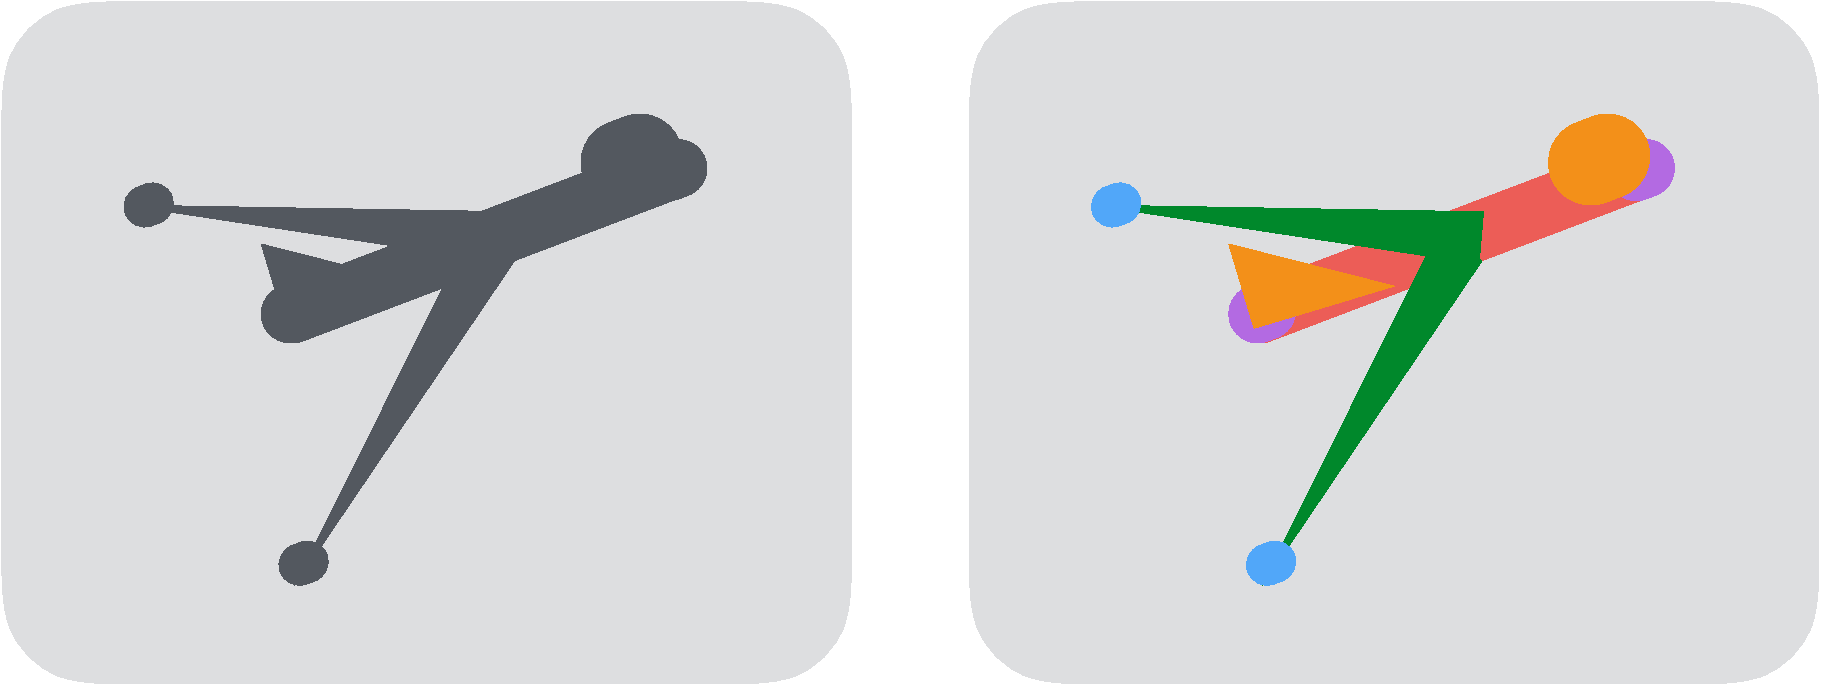
\includegraphics[width=0.7\linewidth]{images/Datenjudo/Bausteine_dplyr_crop} 

}

\caption{Lego-Prinzip: Zerlege eine komplexe Struktur in einfache Bausteine}\label{fig:bausteine}
\end{figure}

\begin{figure}

{\centering 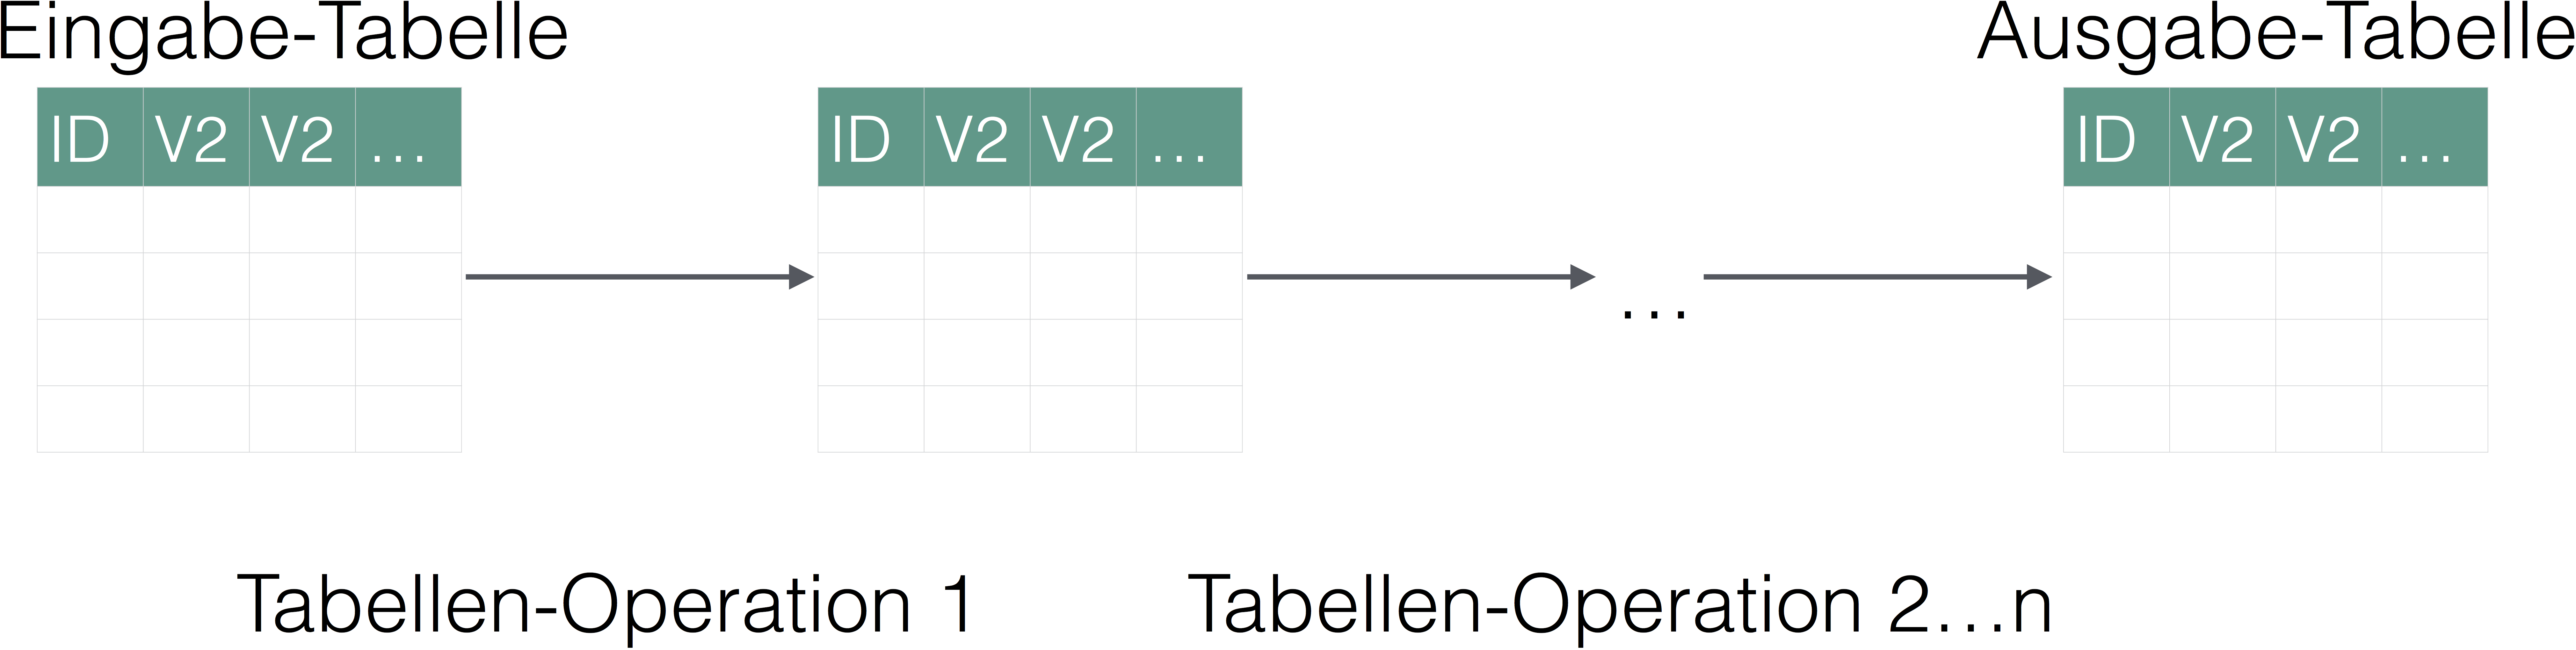
\includegraphics[width=0.7\linewidth]{images/Datenjudo/durchpfeifen_allgemein_crop} 

}

\caption{Durchpfeifen: Ein Dataframe wird von Operation zu Operation weitergereicht}\label{fig:durchpfeifen-allgemein}
\end{figure}

Eine zentrale Idee von \texttt{dplyr} ist, dass es nur ein paar wenige
Grundbausteine geben sollte, die sich gut kombinieren lassen. Sprich:
Wenige grundlegende Funktionen mit eng umgrenzter Funktionalität. Der
Autor, Hadley Wickham, sprach einmal in einem Forum (citation needed),
dass diese Befehle wenig können, das Wenige aber gut. Ein Nachteil
dieser Konzeption kann sein, dass man recht viele dieser Bausteine
kombinieren muss, um zum gewünschten Ergebnis zu kommen. Außerdem muss
man die Logik des Baukastens gut verstanden habe - die Lernkurve ist
also erstmal steiler. Dafür ist man dann nicht darauf angewiesen, dass
es irgendwo ``Mrs Right'' gibt, die genau das kann, was ich will.
Außerdem braucht man sich auch nicht viele Funktionen merken. Es reicht
einen kleinen Satz an Funktionen zu kennen (die praktischerweise
konsistent in Syntax und Methodik sind).

Willkommen in der Welt von \texttt{dyplr}! \texttt{dplyr} hat seinen
Namen, weil es sich ausschließlich um \emph{D}ataframes bemüht; es
erwartet einen Dataframe als Eingabe und gibt einen Dataframe zurück
(zumindest bei den meisten Befehlen).

Diese Bausteine sind typische Tätigkeiten im Umgang mit Daten; nichts
Überraschendes. Schauen wir uns diese Bausteine näher an.

\subsubsection{\texorpdfstring{Zeilen filtern mit
\texttt{filter}}{Zeilen filtern mit filter}}\label{zeilen-filtern-mit-filter}

Häufig will man bestimmte Zeilen aus einer Tabelle filtern;
\texttt{filter}\index{dplyr::filter}. Zum Beispiel man arbeitet für die
Zigarettenindustrie und ist nur an den Rauchern interessiert (die im
Übrigen unser Gesundheitssystem retten (Krämer
\protect\hyperlink{ref-kraemer2011wir}{2011})), nicht an Nicht-Rauchern;
es sollen die nur Umsatzzahlen des letzten Quartals untersucht werden,
nicht die vorherigen Quartale; es sollen nur die Daten aus Labor X
(nicht Labor Y) ausgewertet werden etc.

Abb. \ref{fig:fig-filter} zeigt ein Sinnbild für \texttt{filter}.

\begin{figure}

{\centering 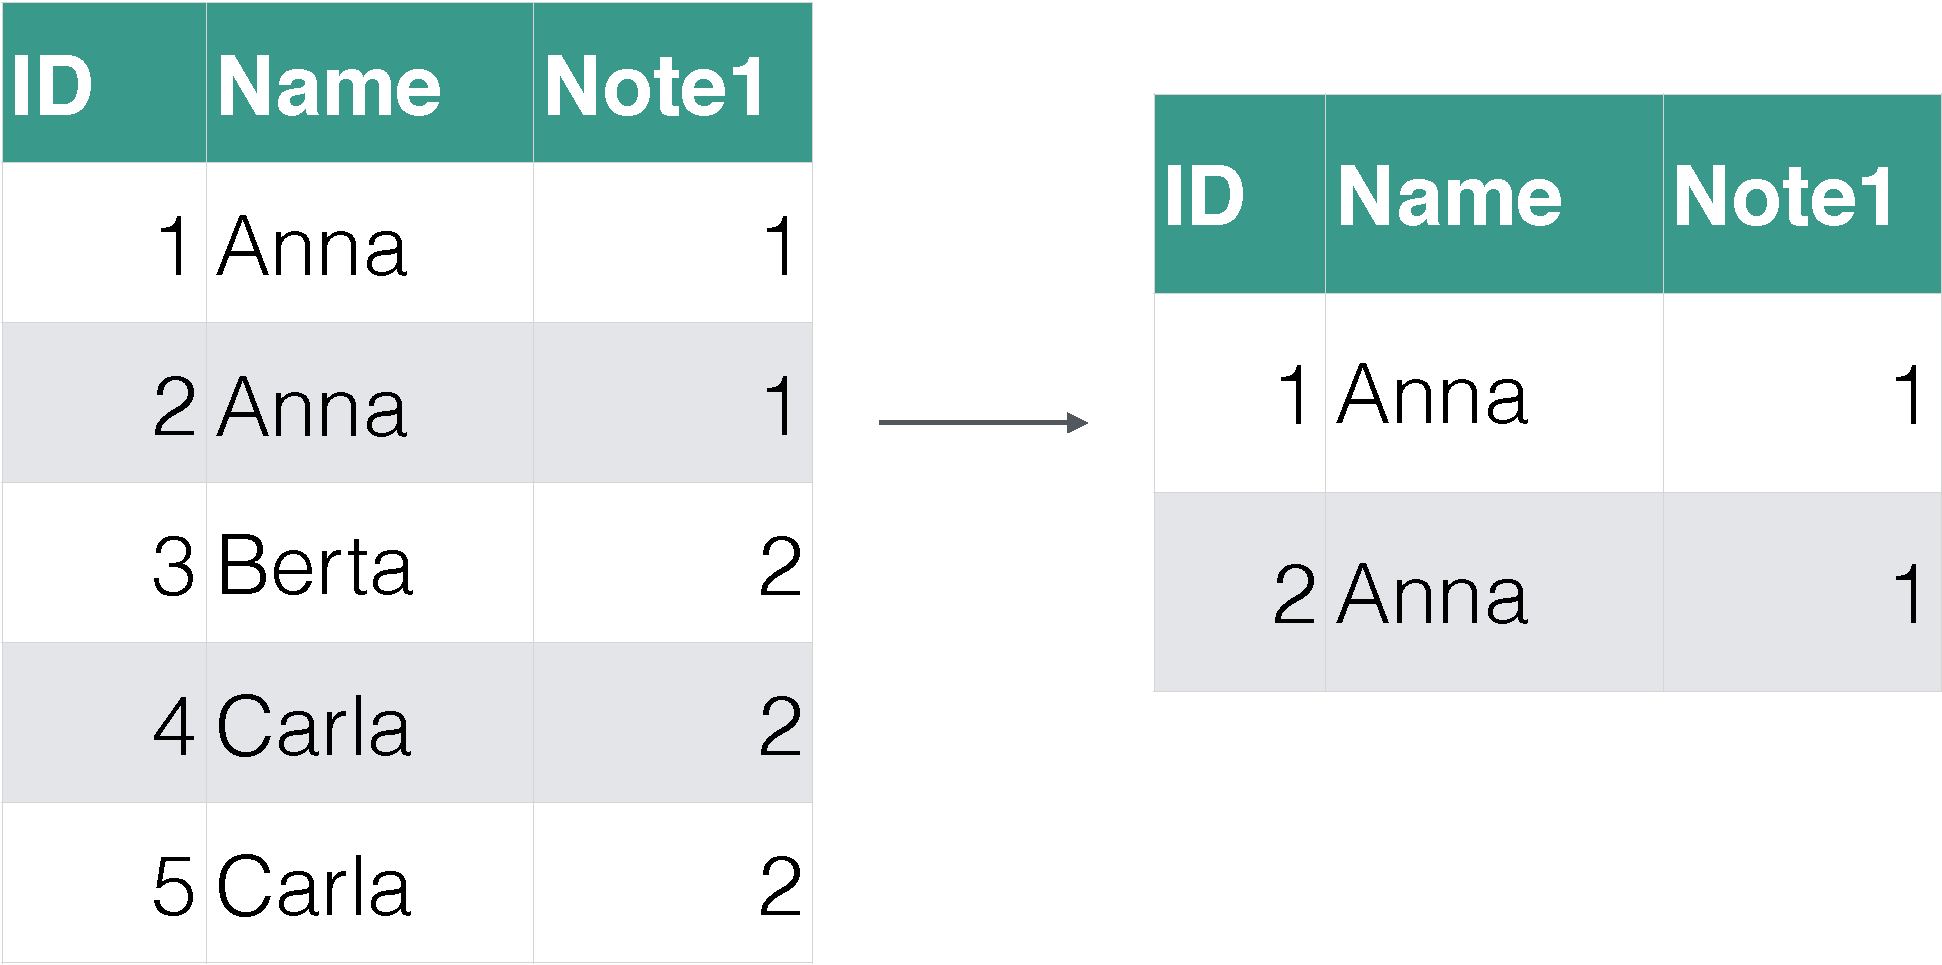
\includegraphics[width=0.7\linewidth]{images/Datenjudo/filter} 

}

\caption{Zeilen filtern}\label{fig:fig-filter}
\end{figure}

Merke:

\begin{quote}
Die Funktion \texttt{filter} filtert Zeilen aus einem Dataframe.
\end{quote}

Schauen wir uns einige Beispiel an; zuerst die Daten laden nicht
vergessen. Achtung: ``Wohnen'' die Daten in einem Paket, muss dieses
Paket installiert sein, damit man auf die Daten zugreifen kann.

\begin{Shaded}
\begin{Highlighting}[]
\KeywordTok{data}\NormalTok{(profiles, }\DataTypeTok{package =} \StringTok{"okcupiddata"}\NormalTok{)  }\CommentTok{# Das Paket muss installiert sein}
\end{Highlighting}
\end{Shaded}

\begin{Shaded}
\begin{Highlighting}[]
\NormalTok{df_frauen <-}\StringTok{ }\KeywordTok{filter}\NormalTok{(profiles, sex ==}\StringTok{ "f"}\NormalTok{)  }\CommentTok{# nur die Frauen}
\NormalTok{df_alt <-}\StringTok{ }\KeywordTok{filter}\NormalTok{(profiles, age >}\StringTok{ }\DecValTok{70}\NormalTok{)  }\CommentTok{# nur die alten Menschen}
\NormalTok{df_alte_frauen <-}\StringTok{ }\KeywordTok{filter}\NormalTok{(profiles, age >}\StringTok{ }\DecValTok{70}\NormalTok{, sex ==}\StringTok{ "f"}\NormalTok{) }
\CommentTok{# nur die alten Frauen, d.h. UND-Verknüpfung}

\NormalTok{df_nosmoke_nodrinks <-}\StringTok{ }\KeywordTok{filter}\NormalTok{(profiles, smokes ==}\StringTok{ "no"} \NormalTok{|}\StringTok{ }\NormalTok{drinks ==}\StringTok{ "not at all"}\NormalTok{) }
\CommentTok{# liefert alle Personen, die Nicht-Raucher *oder* Nicht-Trinker sind}
\end{Highlighting}
\end{Shaded}

Gar nicht so schwer, oder? Allgemeiner gesprochen werden diejenigen
Zeilen gefiltert (also behalten bzw. zurückgeliefert), für die das
Filterkriterium \texttt{TRUE} ist.

\BeginKnitrBlock{rmdcaution}
Manche Befehle wie \texttt{filter} haben einen Allerweltsnamen; gut
möglich, dass ein Befehl mit gleichem Namen in einem anderen (geladenen)
Paket existiert. Das kann dann zu Verwirrungen führen - und kryptischen
Fehlern. Im Zweifel den Namen des richtigen Pakets ergänzen, und zwar
zum Beispiel so: \texttt{dplyr::filter(...)}.
\EndKnitrBlock{rmdcaution}

\paragraph[Aufgaben]{\texorpdfstring{Aufgaben\footnote{F, R, F, F, R}}{Aufgaben}}\label{aufgaben}

\BeginKnitrBlock{rmdexercises}
Richtig oder Falsch!?

\begin{enumerate}
\def\labelenumi{\arabic{enumi}.}
\tightlist
\item
  \texttt{filter} filtert Spalten.
\item
  \texttt{filter} ist eine Funktion aus dem Paket \texttt{dplyr}.
\item
  \texttt{filter} erwartet als ersten Parameter das Filterkriterium.
\item
  \texttt{filter} lässt nur ein Filterkriterium zu.
\item
  Möchte man aus dem Datensatz \texttt{profiles} (\texttt{okcupiddata})
  die Frauen filtern, so ist folgende Syntax korrekt: `filter(profiles,
  sex == ``f'')´.
\end{enumerate}
\EndKnitrBlock{rmdexercises}

\paragraph{\texorpdfstring{Vertiefung: Fortgeschrittene Beispiele für
\texttt{filter}}{Vertiefung: Fortgeschrittene Beispiele für filter}}\label{vertiefung-fortgeschrittene-beispiele-fur-filter}

Einige fortgeschrittene Beispiele für \texttt{filter}:

Man kann alle Elemente (Zeilen) filtern, die zu einer Menge gehören und
zwar mit diesem Operator: \texttt{\%in\%}:

\begin{Shaded}
\begin{Highlighting}[]
\KeywordTok{filter}\NormalTok{(profiles, body_type %in%}\StringTok{ }\KeywordTok{c}\NormalTok{(}\StringTok{"a little extra"}\NormalTok{, }\StringTok{"average"}\NormalTok{))}
\end{Highlighting}
\end{Shaded}

Besonders Textdaten laden zu einigen Extra-Überlegungen ein; sagen wir,
wir wollen alle Personen filtern, die Katzen bei den Haustieren
erwähnen. Es soll reichen, wenn \texttt{cat} ein Teil des Textes ist;
also \texttt{likes\ dogs\ and\ likes\ cats} wäre OK (soll gefiltert
werden). Dazu nutzen wir ein Paket zur Bearbeitung von Strings
(Textdaten):

\begin{Shaded}
\begin{Highlighting}[]

\KeywordTok{filter}\NormalTok{(profiles, }\KeywordTok{str_detect}\NormalTok{(pets, }\StringTok{"cats"}\NormalTok{))}
\end{Highlighting}
\end{Shaded}

Ein häufiger Fall ist, Zeilen \emph{ohne} fehlende Werte (\texttt{NA}s)
zu filtern. Das geht einfach:

\begin{Shaded}
\begin{Highlighting}[]
\NormalTok{profiles_keine_nas <-}\StringTok{ }\KeywordTok{na.omit}\NormalTok{(profiles)}
\end{Highlighting}
\end{Shaded}

Aber was ist, wenn wir nur bei bestimmten Spalten wegen fehlender Werte
besorgt sind? Sagen wir bei \texttt{income} und bei \texttt{sex}:

\begin{Shaded}
\begin{Highlighting}[]
\KeywordTok{filter}\NormalTok{(profiles, !}\KeywordTok{is.na}\NormalTok{(income) |}\StringTok{ }\NormalTok{!}\KeywordTok{is.na}\NormalTok{(sex))}
\end{Highlighting}
\end{Shaded}

\subsubsection{\texorpdfstring{Spalten wählen mit
\texttt{select}}{Spalten wählen mit select}}\label{spalten-wahlen-mit-select}

Das Gegenstück zu \texttt{filter} ist
\texttt{select}\index{dplyr::select}; dieser Befehl liefert die
gewählten Spalten zurück. Das ist häufig praktisch, wenn der Datensatz
sehr ``breit'' ist, also viele Spalten enthält. Dann kann es
übersichtlicher sein, sich nur die relevanten auszuwählen. Abb.
\ref{fig:fig-select} zeigt Sinnbild für diesen Befehl:

\begin{figure}

{\centering 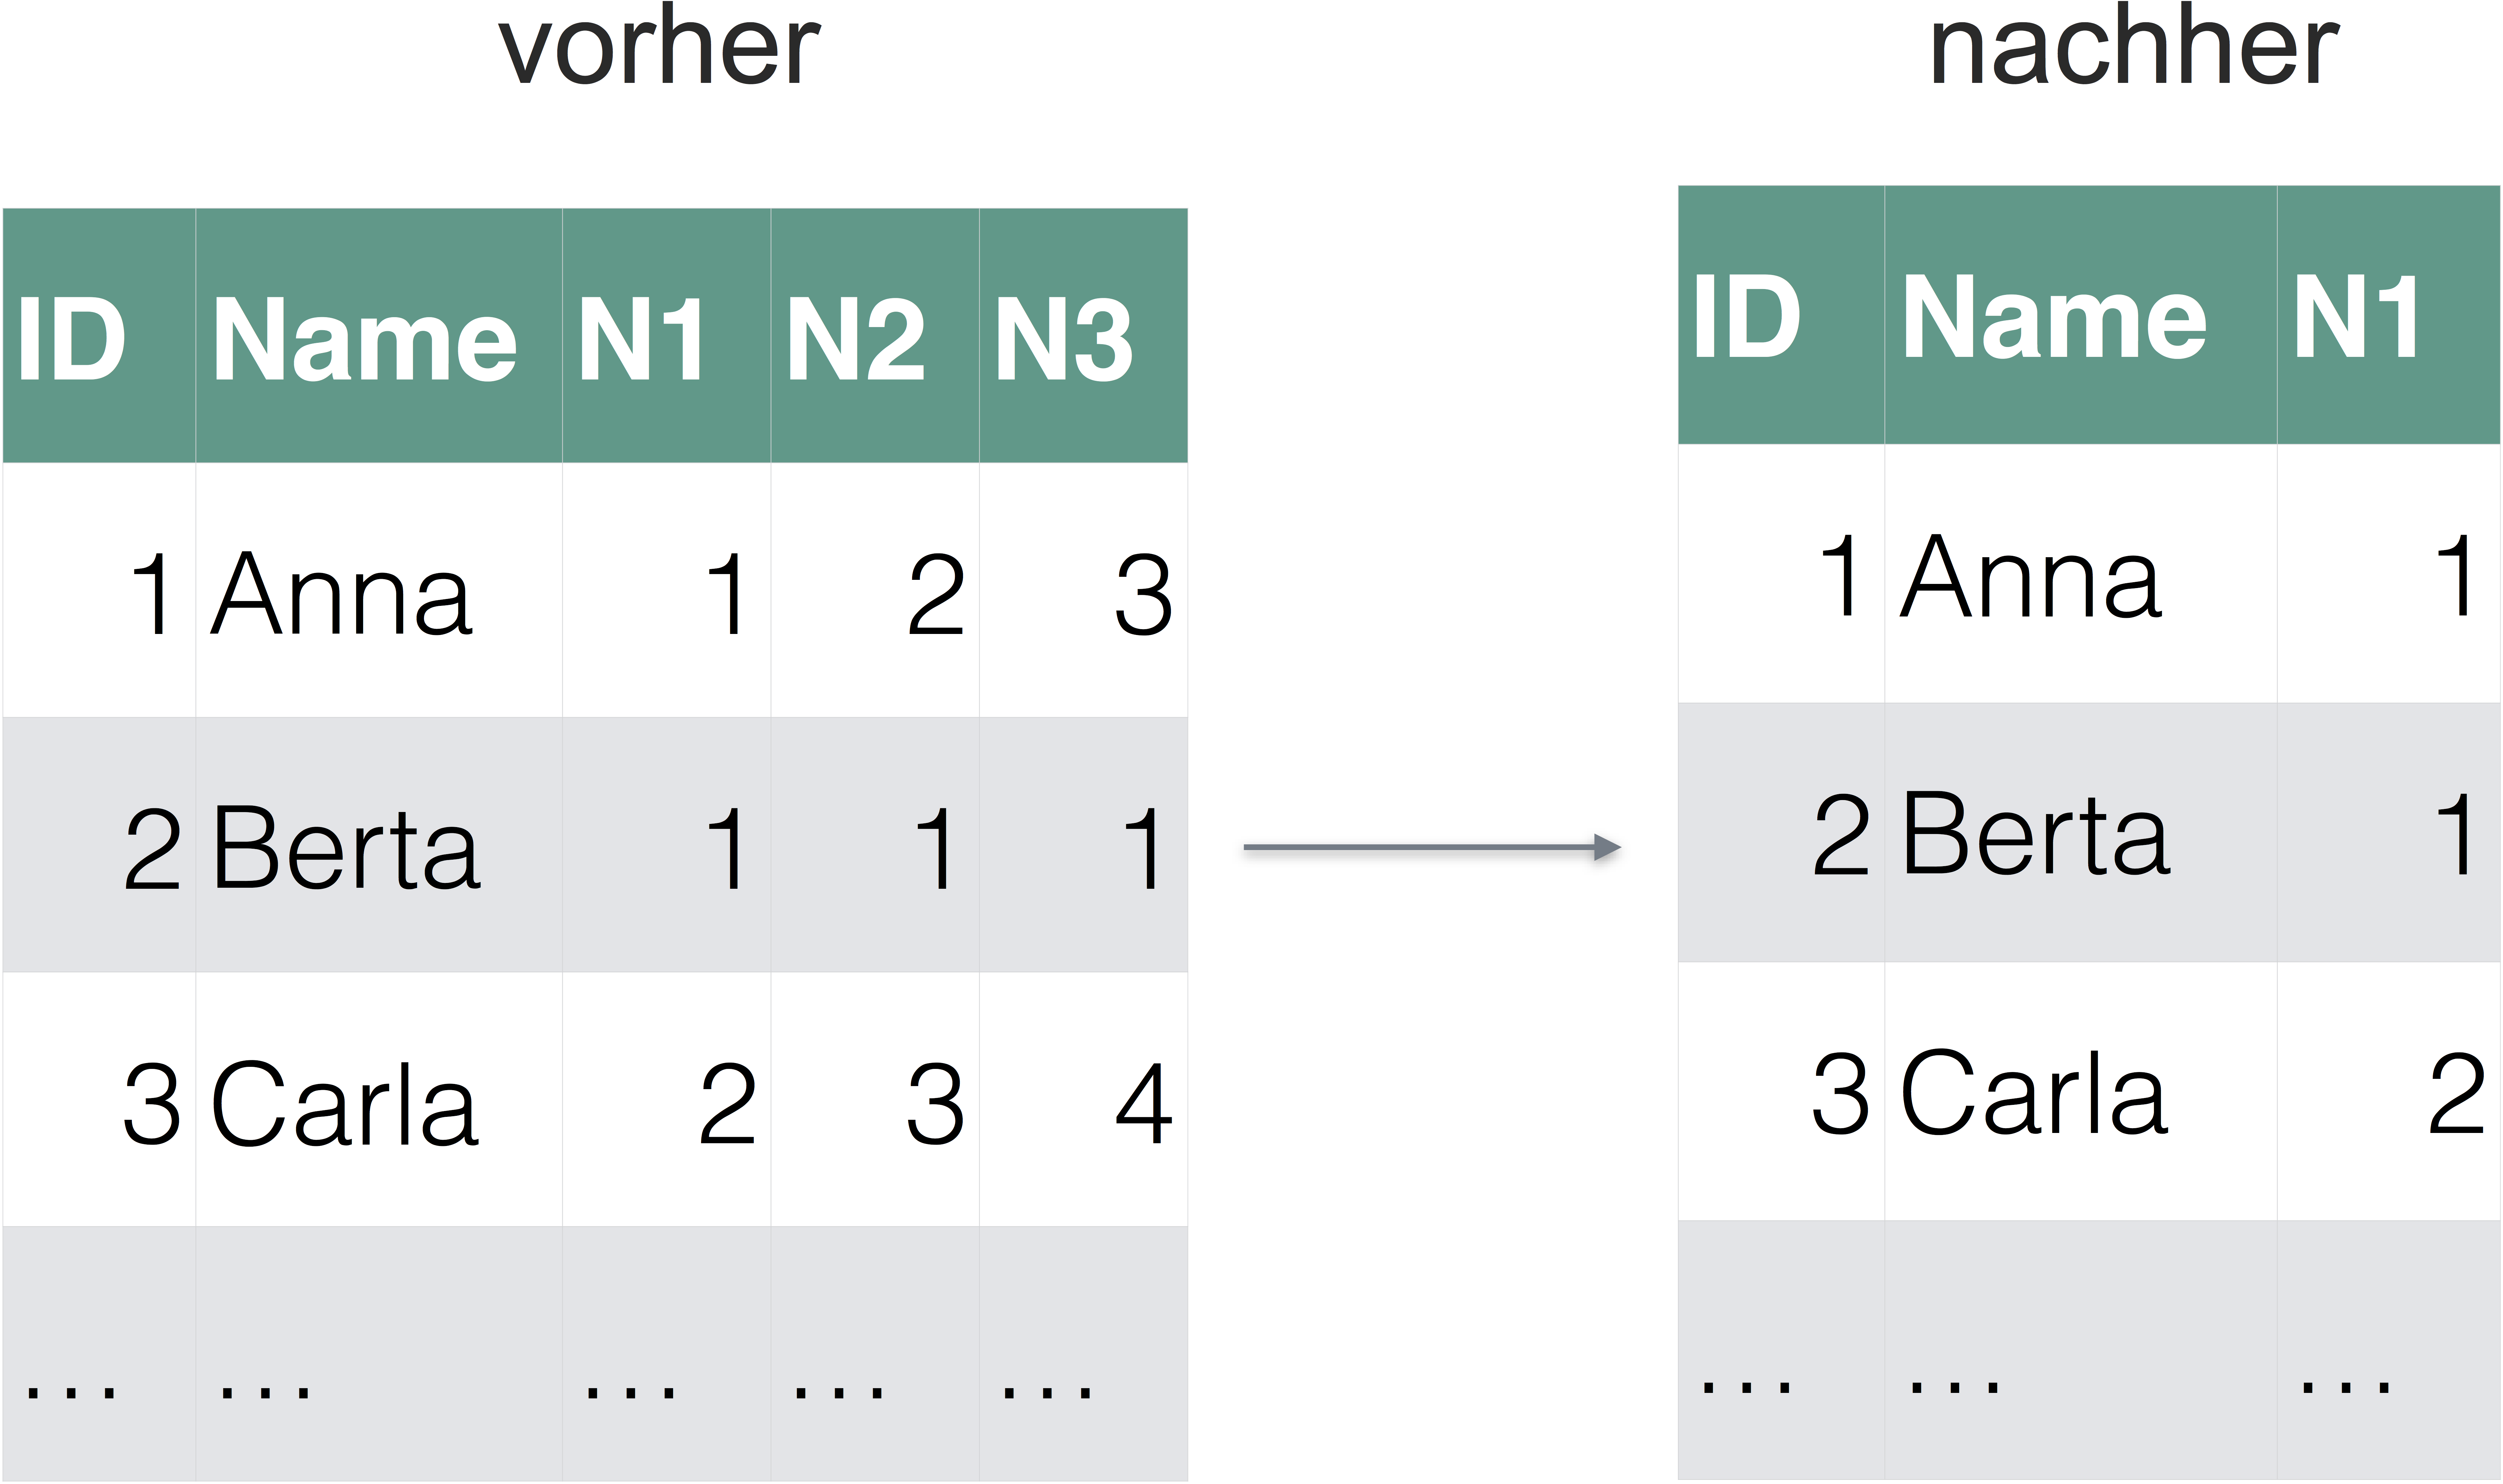
\includegraphics[width=0.7\linewidth]{images/Datenjudo/select} 

}

\caption{Spalten auswählen}\label{fig:fig-select}
\end{figure}

Merke:

\begin{quote}
Die Funktion select wählt Spalten aus einem Dataframe aus.
\end{quote}

Laden wir als ersten einen Datensatz.

\begin{Shaded}
\begin{Highlighting}[]
\NormalTok{stats_test <-}\StringTok{ }\KeywordTok{read.csv}\NormalTok{(}\StringTok{"data/test_inf_short.csv"}\NormalTok{)}
\end{Highlighting}
\end{Shaded}

Dieser Datensatz beinhaltet Daten zu einer Statistikklausur.

Beachten Sie, dass diese Syntax davon ausgeht, dass sich die Daten in
einem Unterordner mit dem Namen \texttt{data} befinden, welcher sich im
Arbeitsverzeichnis befindet\footnote{der angegebene Pfad ist also
  \emph{relativ} zum aktuellen Verzeichnis.}.

\begin{Shaded}
\begin{Highlighting}[]
\KeywordTok{select}\NormalTok{(stats_test, score)  }\CommentTok{# Spalte `score` auswählen}
\KeywordTok{select}\NormalTok{(stats_test, score, study_time)  }
\CommentTok{# Spalten `score` und `study_time` auswählen}

\KeywordTok{select}\NormalTok{(stats_test, score:study_time) }\CommentTok{# dito}
\KeywordTok{select}\NormalTok{(stats_test, }\DecValTok{5}\NormalTok{:}\DecValTok{6}\NormalTok{)  }\CommentTok{# Spalten 5 bis 6 auswählen}
\end{Highlighting}
\end{Shaded}

Tatsächlich ist der Befehl \texttt{select} sehr flexibel; es gibt viele
Möglichkeiten, Spalten auszuwählen. Im \texttt{dplyr}-Cheatsheet findet
sich ein guter Überblick dazu.

\paragraph[Aufgaben]{\texorpdfstring{Aufgaben\footnote{F, F, R, R, F}}{Aufgaben}}\label{aufgaben-1}

\BeginKnitrBlock{rmdexercises}
Richtig oder Falsch!?

\begin{enumerate}
\def\labelenumi{\arabic{enumi}.}
\tightlist
\item
  \texttt{select} wählt \emph{Zeilen} aus.
\item
  \texttt{select} ist eine Funktion aus dem Paket \texttt{knitr}.
\item
  Möchte man zwei Spalten auswählen, so ist folgende Syntax prinzipiell
  korrekt: \texttt{select(df,\ spalte1,\ spalte2)}.
\item
  Möchte man Spalten 1 bis 10 auswählen, so ist folgende Syntax
  prinzipiell korrekt: `select(df, spalte1:spalte10)
\item
  Mit \texttt{select} können Spalten nur bei ihrem Namen, aber nicht bei
  ihrer Nummer aufgerufen werden.
\end{enumerate}
\EndKnitrBlock{rmdexercises}

\subsubsection{\texorpdfstring{Zeilen sortieren mit
\texttt{arrange}}{Zeilen sortieren mit arrange}}\label{zeilen-sortieren-mit-arrange}

Man kann zwei Arten des Umgangs mit R unterscheiden: Zum einen der
``interaktive Gebrauch'' und zum anderen ``richtiges Programmieren''. Im
interaktiven Gebrauch geht es uns darum, die Fragen zum aktuell
vorliegenden Datensatz (schnell) zu beantworten. Es geht nicht darum,
eine allgemeine Lösung zu entwickeln, die wir in die Welt verschicken
können und die dort ein bestimmtes Problem löst, ohne dass der
Entwickler (wir) dabei Hilfestellung geben muss. ``Richtige'' Software,
wie ein R-Paket oder Microsoft Powerpoint, muss diese Erwartung
erfüllen; ``richtiges Programmieren'' ist dazu vonnöten. Natürlich sind
in diesem Fall die Ansprüche an die Syntax (der ``Code'', hört sich
cooler an) viel höher. In dem Fall muss man alle Eventualitäten
voraussehen und sicherstellen, dass das Programm auch beim
merkwürdigsten Nutzer brav seinen Dienst tut. Wir haben hier, beim
interaktiven Gebrauch, niedrigere Ansprüche bzw. andere Ziele.

Beim interaktiven Gebrauch von R (oder beliebigen Analyseprogrammen) ist
das Sortieren von Zeilen eine recht häufige Tätigkeit. Typisches
Beispiel wäre der Lehrer, der eine Tabelle mit Noten hat und wissen
will, welche Schüler die schlechtesten oder die besten sind in einem
bestimmten Fach. Oder bei der Prüfung der Umsätze nach Filialen möchten
wir die umsatzstärksten sowie -schwächsten Niederlassungen kennen.

Ein R-Befehl hierzu ist \texttt{arrange}\index{dplyr::arrange}; einige
Beispiele zeigen die Funktionsweise am besten:

\begin{Shaded}
\begin{Highlighting}[]

\KeywordTok{arrange}\NormalTok{(stats_test, score) }\CommentTok{# liefert die *schlechtesten* Noten zuerst zurück}
\KeywordTok{arrange}\NormalTok{(stats_test, -score) }\CommentTok{# liefert die *besten* Noten zuerst zurück}
\KeywordTok{arrange}\NormalTok{(stats_test, interest, score)}
\end{Highlighting}
\end{Shaded}

\begin{verbatim}
#>     X                 V_1 study_time self_eval interest score
#> 1 234 23.01.2017 18:13:15          3         1        1    17
#> 2   4 06.01.2017 09:58:05          2         3        2    18
#> 3 131 19.01.2017 18:03:45          2         3        4    18
#> 4 142 19.01.2017 19:02:12          3         4        1    18
#> 5  35 12.01.2017 19:04:43          1         2        3    19
#> 6  71 15.01.2017 15:03:29          3         3        3    20
#>    X                 V_1 study_time self_eval interest score
#> 1  3 05.01.2017 23:33:47          5        10        6    40
#> 2  7 06.01.2017 14:25:49         NA        NA       NA    40
#> 3 29 12.01.2017 09:48:16          4        10        3    40
#> 4 41 13.01.2017 12:07:29          4        10        3    40
#> 5 58 14.01.2017 15:43:01          3         8        2    40
#> 6 83 16.01.2017 10:16:52         NA        NA       NA    40
#>     X                 V_1 study_time self_eval interest score
#> 1 234 23.01.2017 18:13:15          3         1        1    17
#> 2 142 19.01.2017 19:02:12          3         4        1    18
#> 3 221 23.01.2017 11:40:30          1         1        1    23
#> 4 230 23.01.2017 16:27:49          1         1        1    23
#> 5  92 17.01.2017 17:18:55          1         1        1    24
#> 6 107 18.01.2017 16:01:36          3         2        1    24
\end{verbatim}

Einige Anmerkungen. Die generelle Syntax lautet
\texttt{arrange(df,\ Spalte1,\ ...)}, wobei \texttt{df} den Dataframe
bezeichnet und \texttt{Spalte1} die erste zu sortierende Spalte; die
Punkte \texttt{...} geben an, dass man weitere Parameter übergeben kann.
Man kann sowohl numerische Spalten als auch Textspalten sortieren. Am
wichtigsten ist hier, dass man weitere Spalten übergeben kann. Dazu
gleich mehr.

Standardmäßig sortiert \texttt{arrange} \emph{aufsteigend} (weil kleine
Zahlen im Zahlenstrahl vor den großen Zahlen kommen). Möchte man diese
Reihenfolge umdrehen (große Werte zuert, d.h. \emph{absteigend}), so
kann man ein Minuszeichen vor den Namen der Spalte setzen.

Gibt man \emph{zwei oder mehr} Spalten an, so werden pro Wert von
\texttt{Spalte1} die Werte von \texttt{Spalte2} sortiert etc; man
betrachte den Output des Beispiels oben dazu.

Merke:

\begin{quote}
Die Funktion arrange sortiert die Zeilen eines Datafames.
\end{quote}

Ein Sinnbild zur Verdeutlichung (s. Abb. \ref{fig:fig-arrange}):

\begin{figure}

{\centering 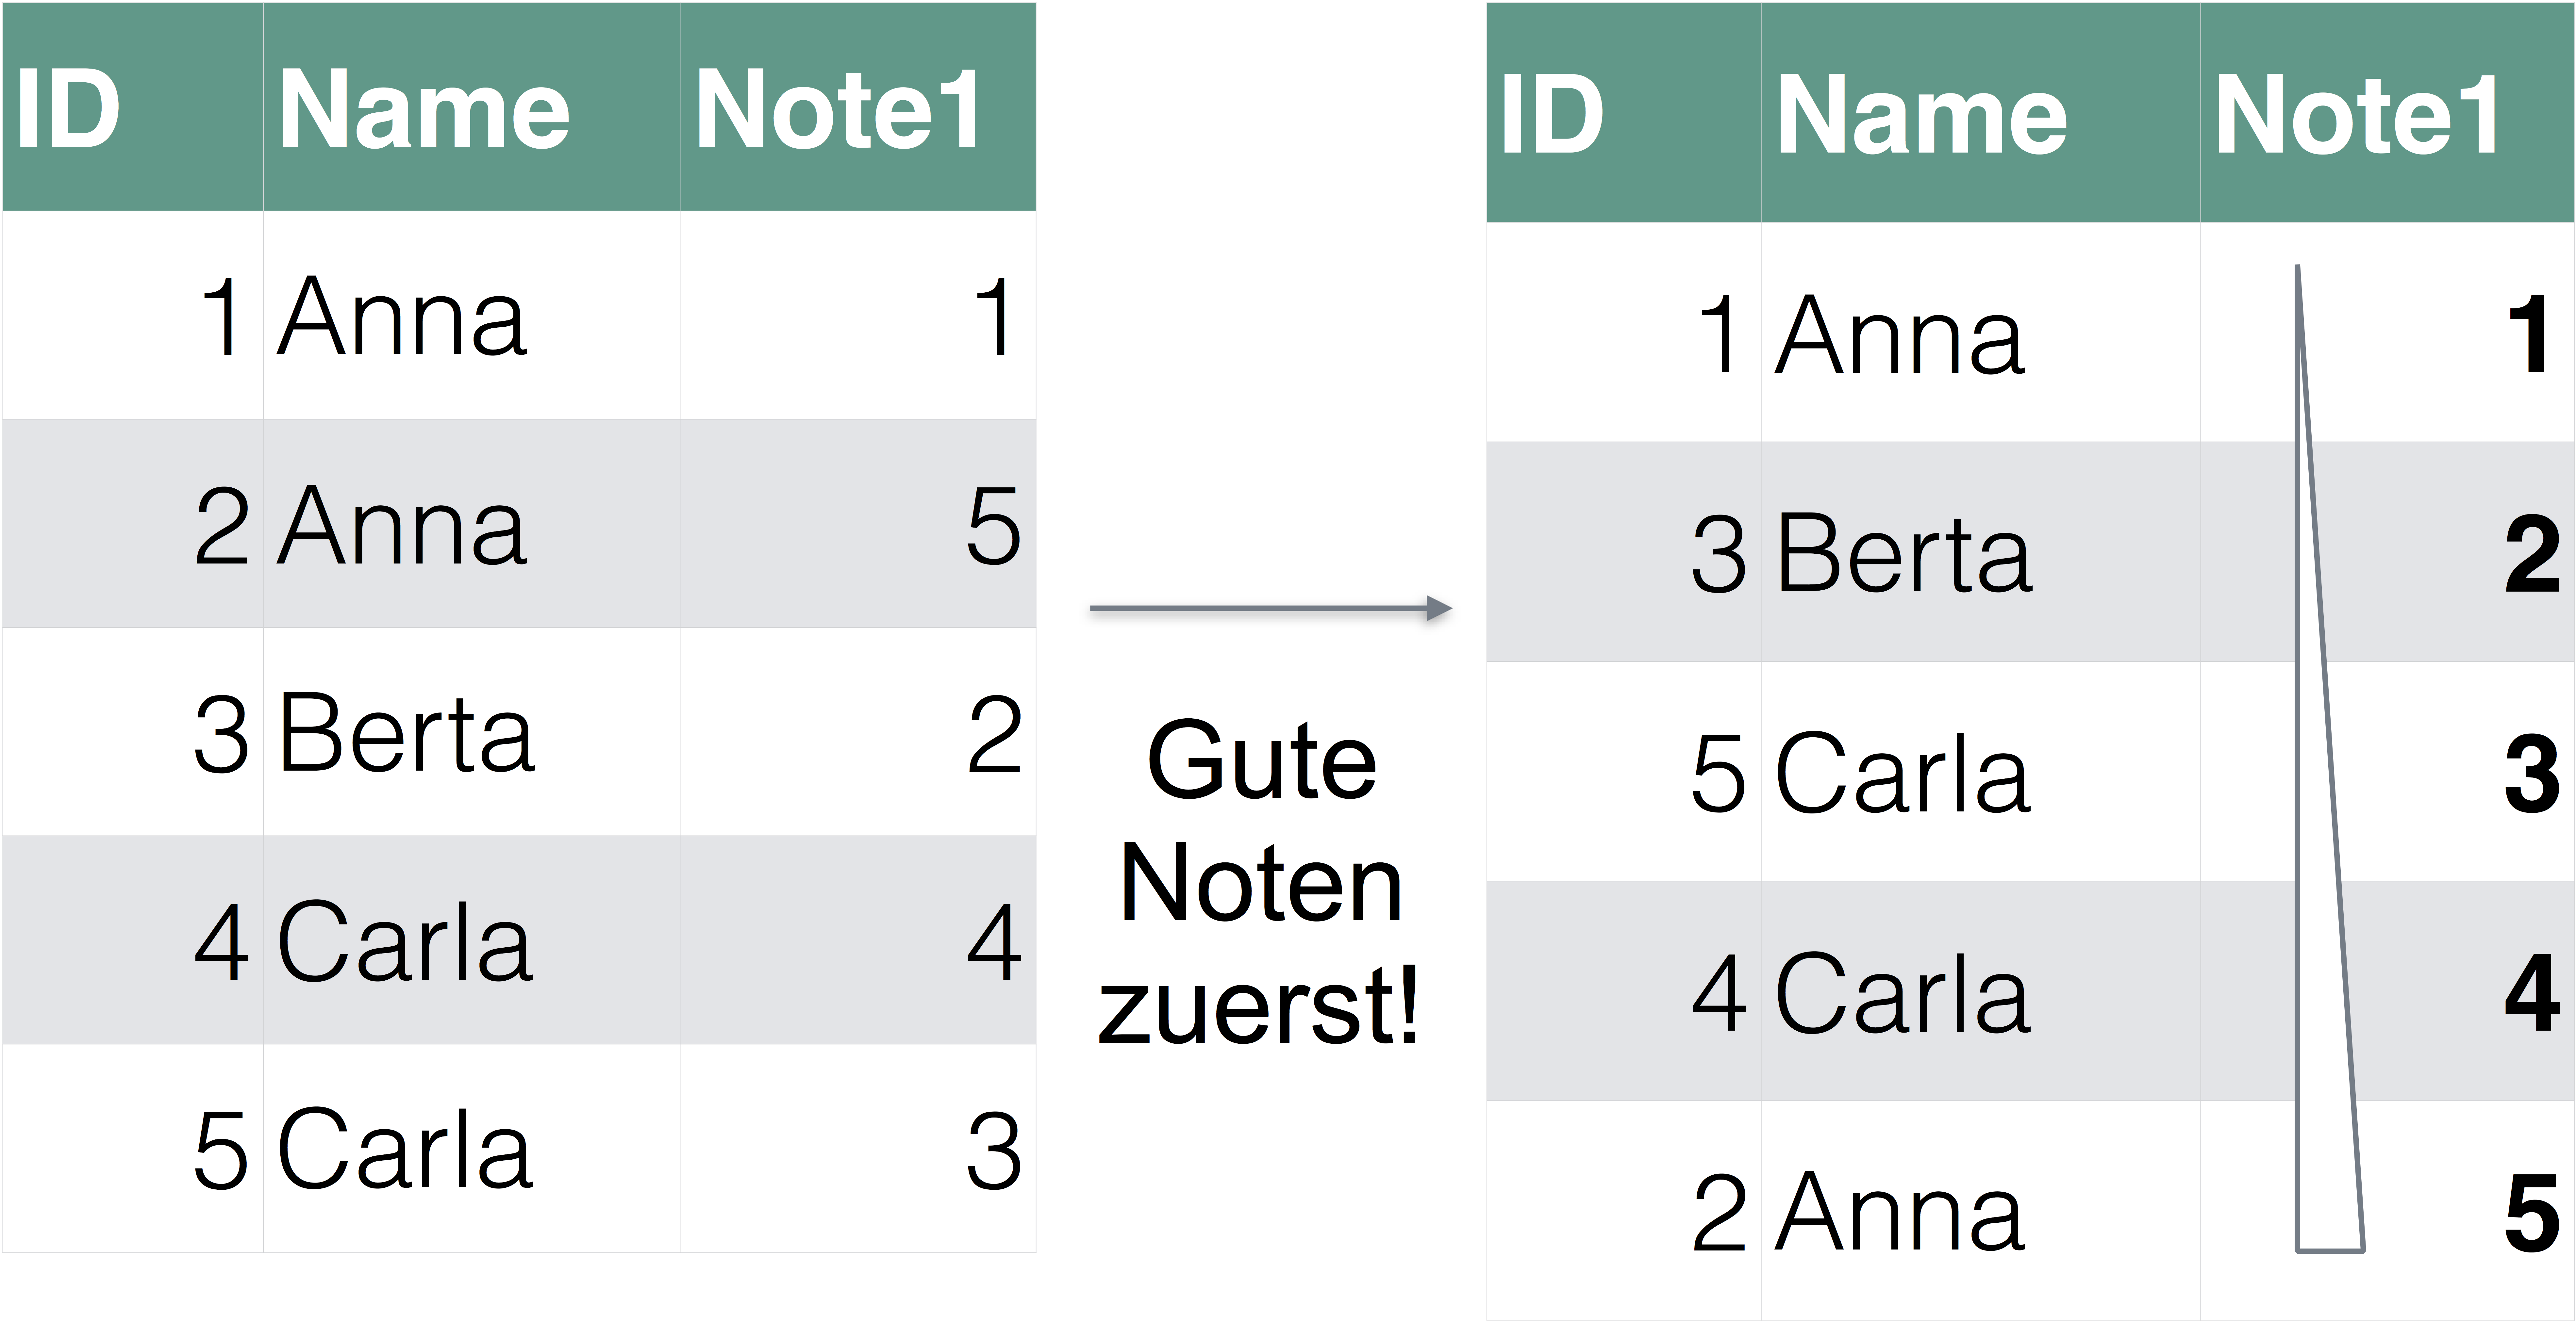
\includegraphics[width=0.7\linewidth]{images/Datenjudo/arrange-crop} 

}

\caption{Spalten sortieren}\label{fig:fig-arrange}
\end{figure}

Ein ähnliches Ergebnis erhält mit man \texttt{top\_n()}, welches die
\texttt{n} \emph{größten Ränge} widergibt:

\begin{Shaded}
\begin{Highlighting}[]

\KeywordTok{top_n}\NormalTok{(stats_test, }\DecValTok{3}\NormalTok{)}
\CommentTok{#>      X                 V_1 study_time self_eval interest score}
\CommentTok{#> 1    3 05.01.2017 23:33:47          5        10        6    40}
\CommentTok{#> 2    7 06.01.2017 14:25:49         NA        NA       NA    40}
\CommentTok{#> 3   29 12.01.2017 09:48:16          4        10        3    40}
\CommentTok{#> 4   41 13.01.2017 12:07:29          4        10        3    40}
\CommentTok{#> 5   58 14.01.2017 15:43:01          3         8        2    40}
\CommentTok{#> 6   83 16.01.2017 10:16:52         NA        NA       NA    40}
\CommentTok{#> 7  116 18.01.2017 23:07:32          4         8        5    40}
\CommentTok{#> 8  119 19.01.2017 09:05:01         NA        NA       NA    40}
\CommentTok{#> 9  132 19.01.2017 18:22:32         NA        NA       NA    40}
\CommentTok{#> 10 175 20.01.2017 23:03:36          5        10        5    40}
\CommentTok{#> 11 179 21.01.2017 07:40:05          5         9        1    40}
\CommentTok{#> 12 185 21.01.2017 15:01:26          4        10        5    40}
\CommentTok{#> 13 196 22.01.2017 13:38:56          4        10        5    40}
\CommentTok{#> 14 197 22.01.2017 14:55:17          4        10        5    40}
\CommentTok{#> 15 248 24.01.2017 16:29:45          2        10        2    40}
\CommentTok{#> 16 249 24.01.2017 17:19:54         NA        NA       NA    40}
\CommentTok{#> 17 257 25.01.2017 10:44:34          2         9        3    40}
\CommentTok{#> 18 306 27.01.2017 11:29:48          4         9        3    40}
\KeywordTok{top_n}\NormalTok{(stats_test, }\DecValTok{3}\NormalTok{, interest)}
\CommentTok{#>     X                 V_1 study_time self_eval interest score}
\CommentTok{#> 1   3 05.01.2017 23:33:47          5        10        6    40}
\CommentTok{#> 2   5 06.01.2017 14:13:08          4         8        6    34}
\CommentTok{#> 3  43 13.01.2017 14:14:16          4         8        6    36}
\CommentTok{#> 4  65 15.01.2017 12:41:27          3         6        6    22}
\CommentTok{#> 5 110 18.01.2017 18:53:02          5         8        6    37}
\CommentTok{#> 6 136 19.01.2017 18:22:57          3         1        6    39}
\CommentTok{#> 7 172 20.01.2017 20:42:46          5        10        6    34}
\CommentTok{#> 8 214 22.01.2017 21:57:36          2         6        6    31}
\CommentTok{#> 9 301 27.01.2017 08:17:59          4         8        6    33}
\end{Highlighting}
\end{Shaded}

Gibt man \emph{keine} Spalte an, so bezieht sich \texttt{top\_n} auf die
letzte Spalte im Datensatz.

Da sich hier mehrere Personen den größten Rang (Wert 40) teilen,
bekommen wir \emph{nicht} 3 Zeilen zurückgeliefert, sondern entsprechend
mehr.

\paragraph[Aufgaben]{\texorpdfstring{Aufgaben\footnote{F, F, F, F, R}}{Aufgaben}}\label{aufgaben-2}

\BeginKnitrBlock{rmdexercises}
Richtig oder Falsch!?

\begin{enumerate}
\def\labelenumi{\arabic{enumi}.}
\tightlist
\item
  \texttt{arrange} arrangiert Spalten.
\item
  \texttt{arrange} sortiert im Standard absteigend.
\item
  \texttt{arrange} lässt nur ein Sortierkriterium zu.
\item
  \texttt{arrange} kann numerische Werte, aber nicht Zeichenketten
  sortieren.
\item
  \texttt{top\_n(5)} liefert die fünf kleinsten Ränge.
\end{enumerate}
\EndKnitrBlock{rmdexercises}

\subsubsection{\texorpdfstring{Datensatz gruppieren mit
\texttt{group\_by}}{Datensatz gruppieren mit group\_by}}\label{datensatz-gruppieren-mit-group_by}

Einen Datensatz zu gruppieren ist eine häufige Angelegenheit: Was ist
der mittlere Umsatz in Region X im Vergleich zu Region Y? Ist die
Reaktionszeit in der Experimentalgruppe kleiner als in der
Kontrollgruppe? Können Männer schneller ausparken als Frauen? Man sieht,
dass das Gruppieren v.a. in Verbindung mit Mittelwerten oder anderen
Zusammenfassungen sinnvol ist; dazu im nächsten Abschnitt mehr.

\begin{quote}
Gruppieren meint, einen Datensatz anhand einer diskreten Variablen (z.B.
Geschlecht) so aufzuteilen, dass Teil-Datensätze entstehen - pro Gruppe
ein Teil-Datensatz (z.B. ein Datensatz, in dem nur Männer enthalten sind
und einer, in dem nur Frauen enthalten sind).
\end{quote}

\begin{figure}

{\centering 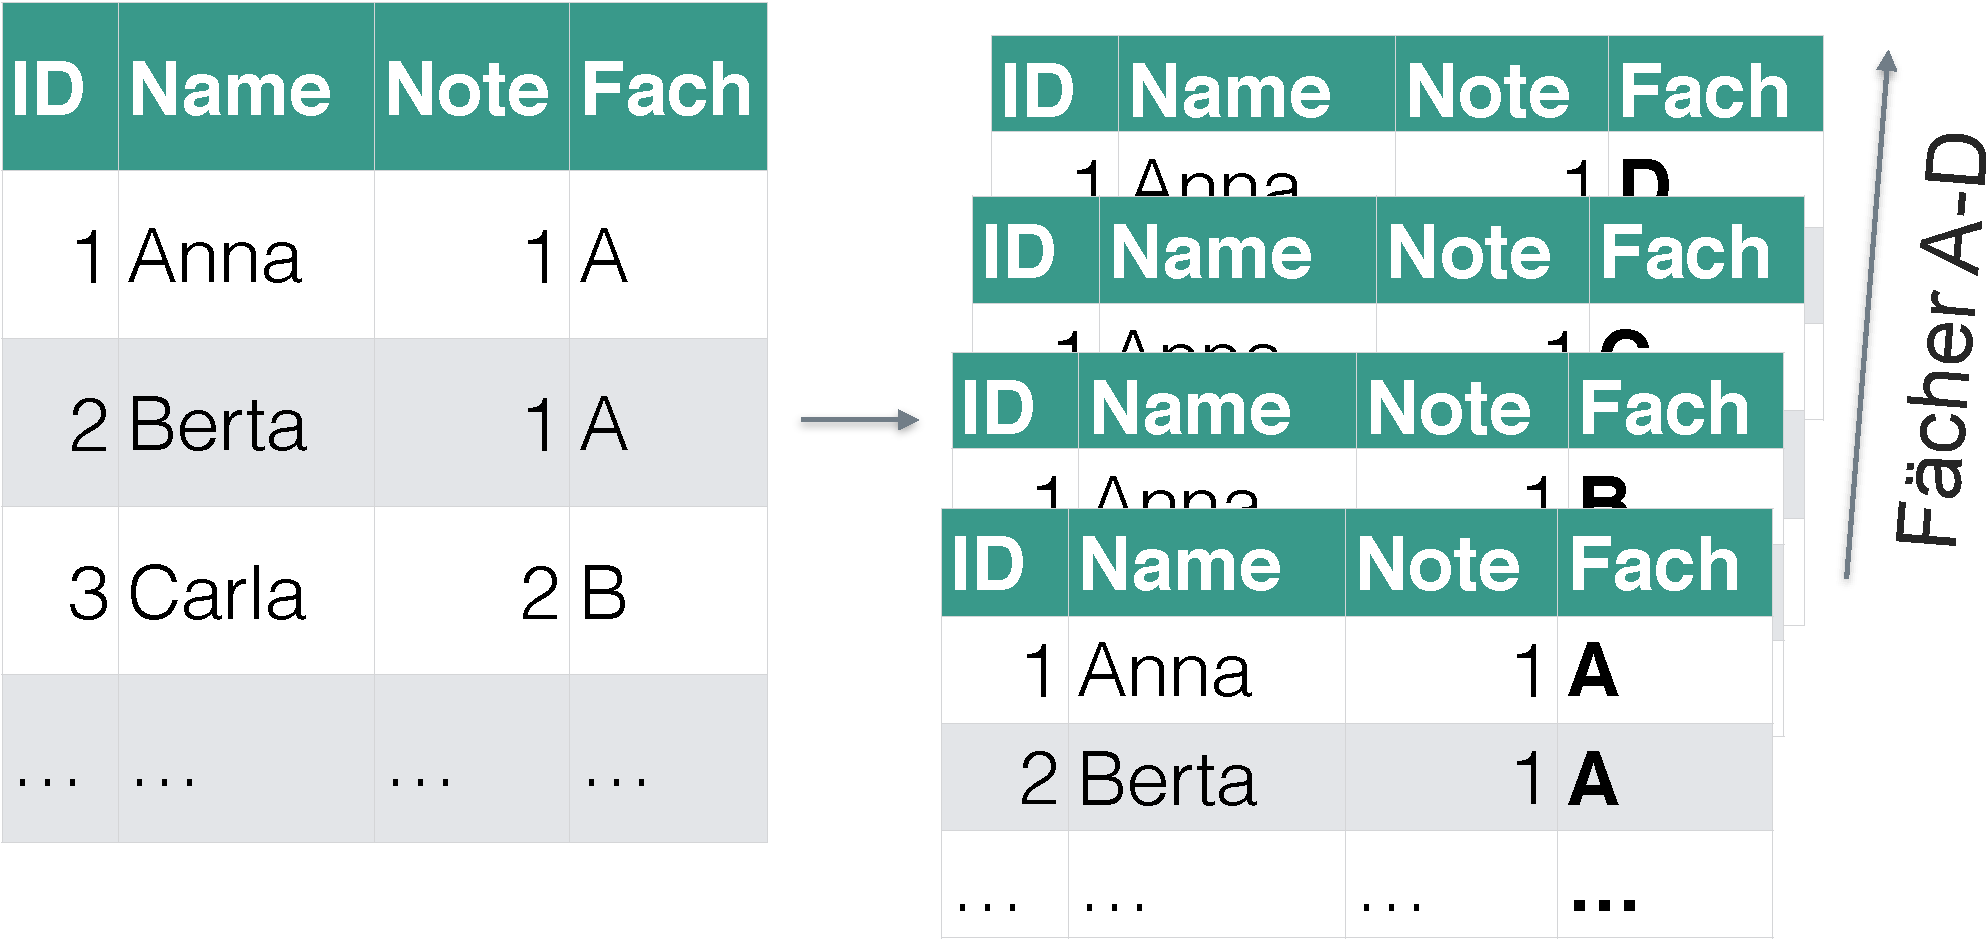
\includegraphics[width=0.7\linewidth]{images/Datenjudo/group_by} 

}

\caption{Datensätze nach Subgruppen aufteilen}\label{fig:fig-groupby}
\end{figure}

In Abbildung \ref{fig:fig-groupby} wurde der Datensatz anhand der Spalte
(d.h. Variable) \texttt{Fach} in mehrere Gruppen geteilt (Fach A, Fach
B\ldots{}). Wir könnten uns als nächstes z.B. Mittelwerte pro Fach -
d.h. pro Gruppe (pro Ausprägung von \texttt{Fach}) - ausgeben lassen; in
diesem Fall vier Gruppen (Fach A bis D).

\begin{Shaded}
\begin{Highlighting}[]
\NormalTok{test_gruppiert <-}\StringTok{ }\KeywordTok{group_by}\NormalTok{(stats_test, interest)}
\NormalTok{test_gruppiert}
\CommentTok{#> Source: local data frame [306 x 6]}
\CommentTok{#> Groups: interest [7]}
\CommentTok{#> }
\CommentTok{#>        X                 V_1 study_time self_eval interest score}
\CommentTok{#>    <int>              <fctr>      <int>     <int>    <int> <int>}
\CommentTok{#> 1      1 05.01.2017 13:57:01          5         8        5    29}
\CommentTok{#> 2      2 05.01.2017 21:07:56          3         7        3    29}
\CommentTok{#> 3      3 05.01.2017 23:33:47          5        10        6    40}
\CommentTok{#> 4      4 06.01.2017 09:58:05          2         3        2    18}
\CommentTok{#> 5      5 06.01.2017 14:13:08          4         8        6    34}
\CommentTok{#> 6      6 06.01.2017 14:21:18         NA        NA       NA    39}
\CommentTok{#> 7      7 06.01.2017 14:25:49         NA        NA       NA    40}
\CommentTok{#> 8      8 06.01.2017 17:24:53          2         5        3    24}
\CommentTok{#> 9      9 07.01.2017 10:11:17          2         3        5    25}
\CommentTok{#> 10    10 07.01.2017 18:10:05          4         5        5    33}
\CommentTok{#> # ... with 296 more rows}
\end{Highlighting}
\end{Shaded}

Schaut man sich nun den Datensatz an, sieht man erstmal wenig Effekt der
Gruppierung. R teilt uns lediglich mit
\texttt{Groups:\ interest\ {[}7{]}}, dass es 7 Gruppen gibt, aber es
gibt keine extra Spalte oder sonstige Anzeichen der Gruppierung. Aber
keine Sorge, wenn wir gleich einen Mittelwert ausrechnen, bekommen wir
den Mittelwert pro Gruppe!

Ein paar Hinweise: \texttt{Source:\ local\ data\ frame\ {[}306\ x\ 6{]}}
will sagen, dass die Ausgabe sich auf einen \texttt{tibble}
bezieht\footnote{\url{http://stackoverflow.com/questions/29084380/what-is-the-meaning-of-the-local-data-frame-message-from-dplyrprint-tbl-df}},
also eine bestimmte Art von Dataframe.
\texttt{Groups:\ interest\ {[}7{]}} zeigt, dass der Tibble in 7 Gruppen
- entsprechend der Werte von \texttt{interest} aufgeteilt ist.

\texttt{group\_by} an sich ist nicht wirklich nützlich. Nützlich wird es
erst, wenn man weitere Funktionen auf den gruppierten Datensatz anwendet
- z.B. Mittelwerte ausrechnet (z.B mit \texttt{summarise}, s. unten).
Die nachfolgenden Funktionen (wenn sie aus \texttt{dplyr} kommen),
berücksichtigen nämlich die Gruppierung. So kann man einfach Mittelwerte
pro Gruppe ausrechnen. \texttt{dplyr} kombiniert dann die
Zusammenfassungen (z.B. Mittelwerte) der einzelnen Gruppen in einen
Dataframe und gibt diesen dann aus.

Die Idee des ``Gruppieren - Zusammenfassen - Kombinieren'' ist flexibel;
man kann sie häufig brauchen. Es lohnt sich, diese Idee zu lernen (vgl.
Abb. \ref{fig:sac}).

\begin{figure}

{\centering 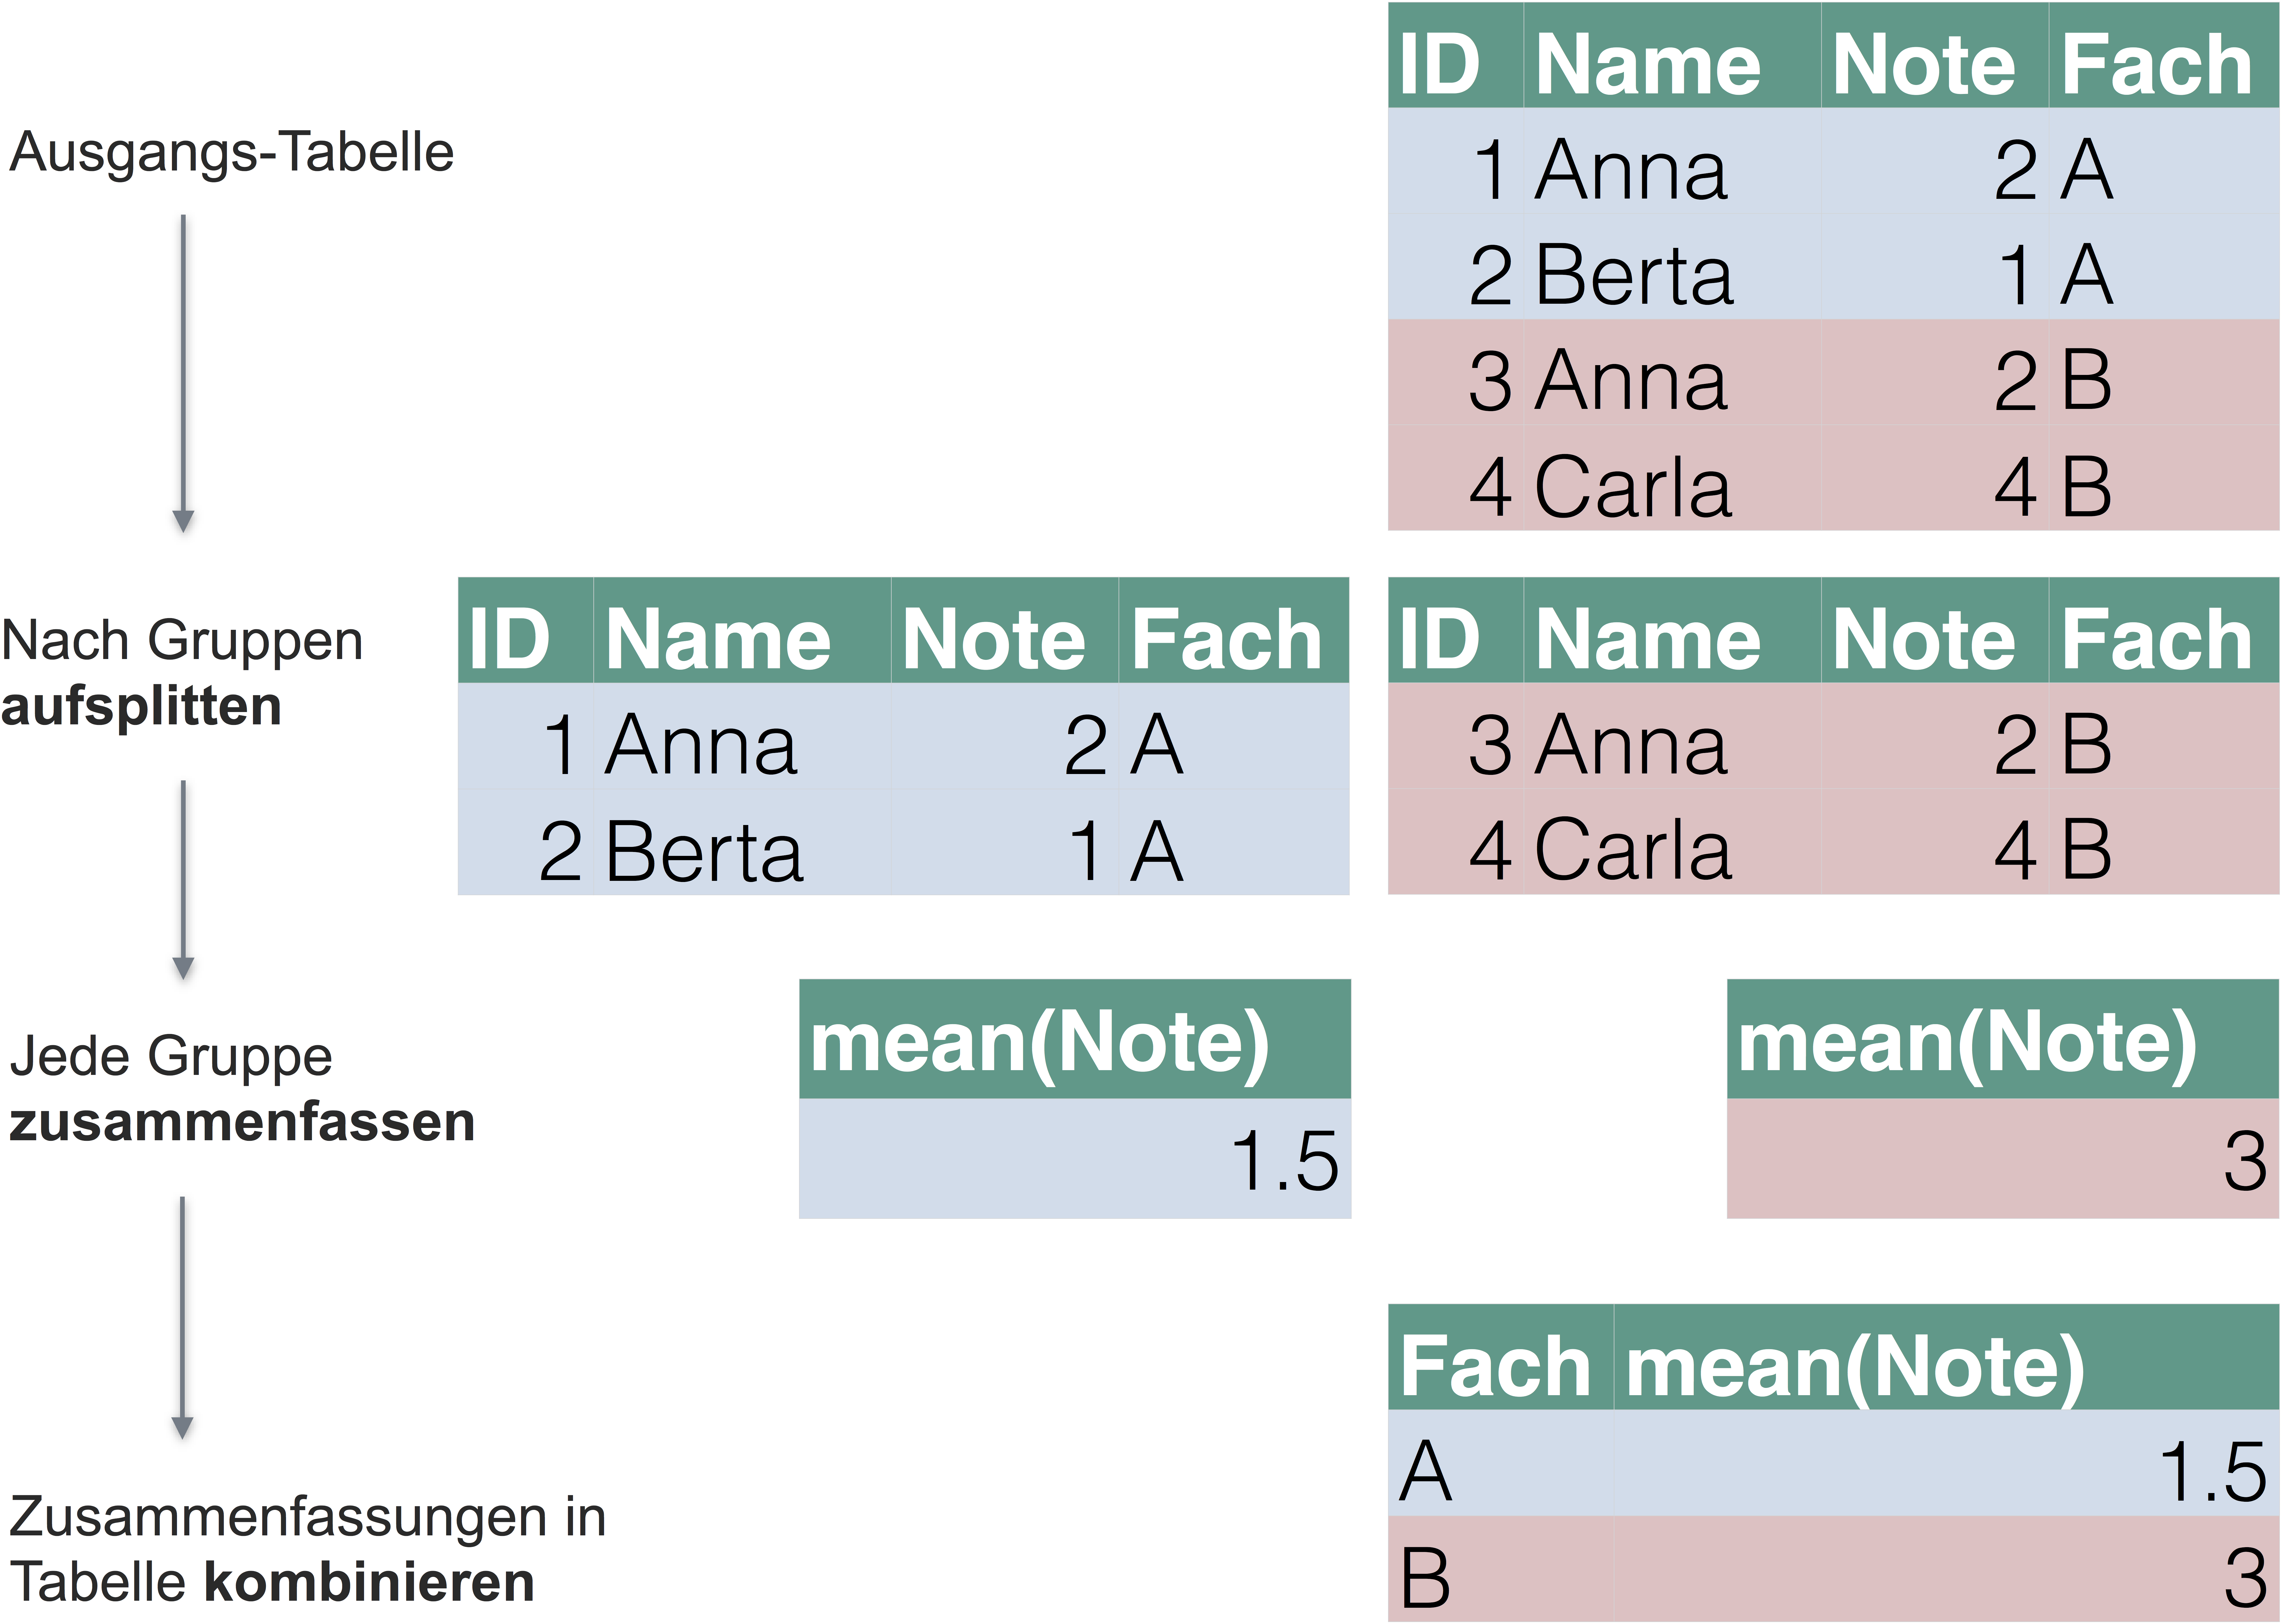
\includegraphics[width=0.7\linewidth]{images/Datenjudo/sac_crop} 

}

\caption{Schematische Darstellung des 'Gruppieren - Zusammenfassen - Kombinieren'}\label{fig:sac}
\end{figure}

\paragraph[Aufgaben]{\texorpdfstring{Aufgaben\footnote{R, F, R, R}}{Aufgaben}}\label{aufgaben-3}

\BeginKnitrBlock{rmdexercises}
Richtig oder Falsch!?

\begin{enumerate}
\def\labelenumi{\arabic{enumi}.}
\tightlist
\item
  Mit \texttt{group\_by} gruppiert man einen Datensatz.
\item
  \texttt{group\_by} lässt nur ein Gruppierungskriterium zu.
\item
  Die Gruppierung durch \texttt{group\_by} wird nur von Funktionen aus
  \texttt{dplyr} erkannt.
\item
  \texttt{group\_by} ist sinnvoll mit \texttt{summarise} zu kombinieren.
\end{enumerate}
\EndKnitrBlock{rmdexercises}

Merke:

\begin{quote}
Mit group\_by teilt man einen Datensatz in Gruppen ein, entsprechend der
Werte einer mehrerer Spalten.
\end{quote}

\subsubsection{\texorpdfstring{Eine Spalte zusammenfassen mit
\texttt{summarise}}{Eine Spalte zusammenfassen mit summarise}}\label{eine-spalte-zusammenfassen-mit-summarise}

Vielleicht die wichtigste oder häufigte Tätigkeit in der Analyse von
Daten ist es, eine Spalte zu \emph{einem} Wert zusammenzufassen;
\texttt{summarise}\index{dplyr::summarise} leistet dies. Anders gesagt:
Einen Mittelwert berechnen, den größten (kleinsten) Wert heraussuchen,
die Korrelation berechnen oder eine beliebige andere Statistik ausgeben
lassen. Die Gemeinsamkeit dieser Operaitonen ist, dass sie eine Spalte
zu einem Wert zusammenfassen, ``aus Spalte mach Zahl'', sozusagen. Daher
ist der Name des Befehls \texttt{summarise} ganz passend. Genauer gesagt
fasst dieser Befehl eine Spalte zu einer Zahl zusammen \emph{anhand}
einer Funktion wie \texttt{mean} oder \texttt{max} (vgl. Abb.
\ref{fig:fig-summarise}. Hierbei ist jede Funktion erlaubt, die eine
Spalte als Input verlangt und eine Zahl zurückgibt; andere Funktionen
sind bei \texttt{summarise} nicht erlaubt.

\begin{figure}

{\centering 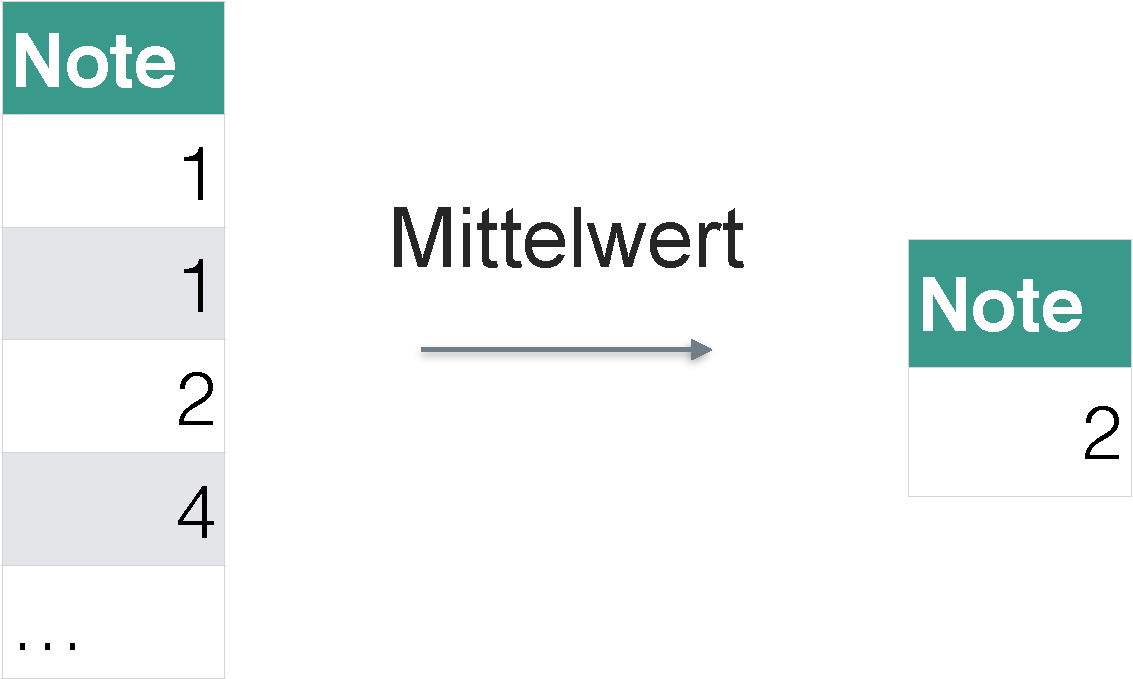
\includegraphics[width=0.7\linewidth]{images/Datenjudo/summarise} 

}

\caption{Spalten zu einer Zahl zusammenfassen}\label{fig:fig-summarise}
\end{figure}

\begin{Shaded}
\begin{Highlighting}[]
\KeywordTok{summarise}\NormalTok{(stats_test, }\KeywordTok{mean}\NormalTok{(score))}
\CommentTok{#>   mean(score)}
\CommentTok{#> 1        31.1}
\end{Highlighting}
\end{Shaded}

Man könnte diesen Befehl so ins Deutsche übersetzen:
\texttt{Fasse\ aus\ Tabelle\ stats\_test\ die\ Spalte\ score\ anhand\ des\ Mittelwerts\ zusammen}.
Nicht vergessen, wenn die Spalte \texttt{score} fehlende Werte hat, wird
der Befehl \texttt{mean} standardmäßig dies mit \texttt{NA} quittieren.
Ergänzt man den Parameter \texttt{nr.rm\ =\ TRUE}, so ignoriert R
fehlende Werte und der Befehl \texttt{mean} liefert ein Ergebnis zurück.

Jetzt können wir auch die Gruppierung nutzen:

\begin{Shaded}
\begin{Highlighting}[]
\NormalTok{test_gruppiert <-}\StringTok{ }\KeywordTok{group_by}\NormalTok{(stats_test, interest)}
\KeywordTok{summarise}\NormalTok{(test_gruppiert, }\KeywordTok{mean}\NormalTok{(score, }\DataTypeTok{na.rm =} \OtherTok{TRUE}\NormalTok{))}
\CommentTok{#> # A tibble: 7 × 2}
\CommentTok{#>   interest `mean(score, na.rm = TRUE)`}
\CommentTok{#>      <int>                       <dbl>}
\CommentTok{#> 1        1                        28.3}
\CommentTok{#> 2        2                        29.7}
\CommentTok{#> 3        3                        30.8}
\CommentTok{#> 4        4                        29.9}
\CommentTok{#> 5        5                        32.5}
\CommentTok{#> 6        6                        34.0}
\CommentTok{#> 7       NA                        33.1}
\end{Highlighting}
\end{Shaded}

Der Befehl \texttt{summarise} erkennt also, wenn eine (mit
\texttt{group\_by}) gruppierte Tabelle vorliegt. Jegliche
Zusammenfassung, die wir anfordern, wird anhand der
Gruppierungsinformation aufgeteilt werden. In dem Beispiel bekommen wir
einen Mittelwert für jeden Wert von \texttt{interest}.
Interessanterweise sehen wir, dass der Mittelwert tendenziell größer
wird, je größer \texttt{interest} wird.

Alle diese \texttt{dplyr}-Befehle geben einen Dataframe zurück, was
praktisch ist für weitere Verarbeitung. In diesem Fall heißen die
Spalten \texttt{interst} und \texttt{mean(score)}. Zweiter Name ist
nicht so schön, daher ändern wir den wie folgt:

Jetzt können wir auch die Gruppierung nutzen:

\begin{Shaded}
\begin{Highlighting}[]
\NormalTok{test_gruppiert <-}\StringTok{ }\KeywordTok{group_by}\NormalTok{(stats_test, interest)}
\KeywordTok{summarise}\NormalTok{(test_gruppiert, }\DataTypeTok{mw_pro_gruppe =} \KeywordTok{mean}\NormalTok{(score, }\DataTypeTok{na.rm =} \OtherTok{TRUE}\NormalTok{))}
\CommentTok{#> # A tibble: 7 × 2}
\CommentTok{#>   interest mw_pro_gruppe}
\CommentTok{#>      <int>         <dbl>}
\CommentTok{#> 1        1          28.3}
\CommentTok{#> 2        2          29.7}
\CommentTok{#> 3        3          30.8}
\CommentTok{#> 4        4          29.9}
\CommentTok{#> 5        5          32.5}
\CommentTok{#> 6        6          34.0}
\CommentTok{#> 7       NA          33.1}
\end{Highlighting}
\end{Shaded}

Nun heißt die zweite Spalte \texttt{mw\_pro\_Gruppe}.
\texttt{na.rm\ =\ TRUE} veranlasst, bei fehlenden Werten trotzdem einen
Mittelwert zurückzuliefern (die Zeilen mit fehlenden Werten werden in
dem Fall ignoriert).

Grundsätzlich ist die Philosophie der \texttt{dplyr}-Befehle: ``Mach nur
eine Sache, aber die dafür gut''. Entsprechend kann \texttt{summarise}
nur \emph{Spalten} zusammenfassen, aber keine \emph{Zeilen}.

Merke:

\begin{quote}
Mit summarise kann man eine Spalte eines Dataframes zu einem Wert
zusammenfassen.
\end{quote}

\paragraph{\texorpdfstring{Deskriptive Statistik mit
\texttt{summarise}}{Deskriptive Statistik mit summarise}}\label{deskriptive-statistik-mit-summarise}

\begin{quote}
Die deskriptive Statistik hat zwei Haupt-Bereiche: Lagemaße und
Streuungsmaße.
\end{quote}

\emph{Lagemaße} geben den ``typischen'', ``mittleren'' oder
``repräsentativen'' Vertreter der Verteilung an. Bei den
Lagemaßen\index{Lagemaße} denkt man sofort an das \emph{arithmetische
Mittel} (synonym: Mittelwert; häufig als \(\bar{X}\) abgekürzt;
\texttt{mean}). Ein Nachteil von Mittelwerten ist, dass sie nicht robust
gegenüber Extremwerte sind: Schon ein vergleichsweise großer Einzelwert
kann den Mittelwert deutlich verändern und damit die Repräsentativität
des Mittelwerts für die Gesamtmenge der Daten in Frage stellen. Eine
robuste Variante ist der \emph{Median} (Md; \texttt{median}). Ist die
Anzahl der (unterschiedlichen) Ausprägungen nicht zu groß im Verhältnis
zur Fallzahl, so ist der \emph{Modus} eine sinnvolle Statistik; er gibt
die häufigste Ausprägung an\footnote{Der \emph{Modus} ist im Standard-R
  nicht mit einem eigenen Befehl vertreten. Man kann ihn aber leicht von
  Hand bestimmen; s.u. Es gibt auch einige Pakete, die diese Funktion
  anbieten: z.B.
  \url{https://cran.r-project.org/web/packages/modes/index.html}}.

\emph{Streuungsmaße}\index{Streuungsmaße} geben die Unterschiedlichkeit
in den Daten wieder; mit anderen Worten: sind die Daten sich ähnlich
oder unterscheiden sich die Werte deutlich? Zentrale Statistiken sind
der \emph{mittlere Absolutabstand} (MAA; MAD),\footnote{Der \emph{MAD}
  ist im Standard-R nicht mit einem eigenen Befehl vertreten. Es gibt
  einige Pakete, die diese Funktion anbieten: z.B.
  \url{https://artax.karlin.mff.cuni.cz/r-help/library/lsr/html/aad.html}}
die \emph{Standardabweichung} (sd; \texttt{sd}), die \emph{Varianz}
(Var; \texttt{var}) und der \emph{Interquartilsabstand} (IQR;
\texttt{IQR}). Da nur der IQR \emph{nicht} auf dem Mittelwert basiert,
ist er am robustesten. Beliebige Quantile bekommt man mit dem R-Befehl
\texttt{quantile}.

Der Befehl \texttt{summarise} eignet sich, um deskriptive Statistiken
auszurechnen.

\begin{Shaded}
\begin{Highlighting}[]
\KeywordTok{summarise}\NormalTok{(stats_test, }\KeywordTok{mean}\NormalTok{(score))}
\CommentTok{#>   mean(score)}
\CommentTok{#> 1        31.1}
\KeywordTok{summarise}\NormalTok{(stats_test, }\KeywordTok{sd}\NormalTok{(score))}
\CommentTok{#>   sd(score)}
\CommentTok{#> 1      5.74}
\end{Highlighting}
\end{Shaded}

Natürlich könnte man auch einfacher schreiben:

\begin{Shaded}
\begin{Highlighting}[]
\KeywordTok{mean}\NormalTok{(stats_test$score)}
\CommentTok{#> [1] 31.1}
\KeywordTok{median}\NormalTok{(stats_test$score)}
\CommentTok{#> [1] 31}
\end{Highlighting}
\end{Shaded}

\texttt{summarise} liefert aber im Unterschied zu \texttt{mean} etc.
immer einen Dataframe zurück. Da der Dataframe die typische
Datenstruktur ist, ist es häufig praktisch, wenn man einen Dataframe
zurückbekommt, mit dem man weiterarbeiten kann. Außerdem lassen
\texttt{mean} etc. keine Gruppierungsoperationen zu; über
\texttt{group\_by} kann man dies aber bei \texttt{dplyr} erreichen.

\paragraph[Aufgaben]{\texorpdfstring{Aufgaben\footnote{R, R, R, R, R}}{Aufgaben}}\label{aufgaben-4}

\BeginKnitrBlock{rmdexercises}
Richtig oder Falsch!?

\begin{enumerate}
\def\labelenumi{\arabic{enumi}.}
\tightlist
\item
  Möchte man aus der Tabelle \texttt{stats\_test} den Mittelwert für die
  Spalte \texttt{score} berechnen, so ist folgende Syntax korrekt:
  \texttt{summarise(stats\_test,\ mean(score))}.
\item
  \texttt{summarise} liefert eine Tabelle, genauer: einen Tibble,
  zurück.
\item
  Die Tabelle, die diese Funktion zurückliefert:
  \texttt{summarise(stats\_test,\ mean(score))}, hat eine Spalte mit dem
  Namen \texttt{mean(score)}.
\item
  \texttt{summarise} lässt zu, dass die zu berechnende Spalte einen
  Namen vom Nutzer zugewiesen bekommt.
\item
  \texttt{summarise} darf nur verwendet werden, wenn eine Spalte zu
  einem Wert zusammengefasst werden soll.
\end{enumerate}
\EndKnitrBlock{rmdexercises}

\begin{enumerate}
\def\labelenumi{\arabic{enumi}.}
\tightlist
\item
  (Fortgeschritten) Bauen Sie einen eigenen Weg, um den mittleren
  Absolutabstand auszurechnen! Gehen Sie der Einfachheit halber (zuerst)
  von einem Vektor mit den Werten (1,2,3) aus!
\end{enumerate}

Lösung:

\begin{Shaded}
\begin{Highlighting}[]
\NormalTok{x <-}\StringTok{ }\KeywordTok{c}\NormalTok{(}\DecValTok{1}\NormalTok{, }\DecValTok{2}\NormalTok{, }\DecValTok{3}\NormalTok{)}
\NormalTok{x_mw <-}\StringTok{ }\KeywordTok{mean}\NormalTok{(x)}
\NormalTok{x_delta <-}\StringTok{ }\NormalTok{x -}\StringTok{ }\NormalTok{x_mw}
\NormalTok{x_delta <-}\StringTok{ }\KeywordTok{abs}\NormalTok{(x_delta)}
\NormalTok{mad <-}\StringTok{ }\KeywordTok{mean}\NormalTok{(x_delta)}
\NormalTok{mad}
\CommentTok{#> [1] 0.667}
\end{Highlighting}
\end{Shaded}

\subsubsection{\texorpdfstring{Zeilen zählen mit \texttt{n} und
\texttt{count}}{Zeilen zählen mit n und count}}\label{zeilen-zahlen-mit-n-und-count}

Ebenfalls nützlich ist es, Zeilen zu zählen. Im Gegensatz zum
Standardbefehl\footnote{Standardbefehl meint, dass die Funktion zum
  Standardrepertoire von R gehört, also nicht über ein Paket extra
  geladen werden muss} \texttt{nrow} versteht der \texttt{dyplr}-Befehl
\texttt{n}\index{dplyr::n} auch Gruppierungen. \texttt{n} darf nur
innerhalb von \texttt{summarise} oder ähnlichen \texttt{dplyr}-Befehlen
verwendet werden.

\begin{Shaded}
\begin{Highlighting}[]
\KeywordTok{summarise}\NormalTok{(stats_test, }\KeywordTok{n}\NormalTok{())}
\CommentTok{#>   n()}
\CommentTok{#> 1 306}
\KeywordTok{summarise}\NormalTok{(test_gruppiert, }\KeywordTok{n}\NormalTok{())}
\CommentTok{#> # A tibble: 7 × 2}
\CommentTok{#>   interest `n()`}
\CommentTok{#>      <int> <int>}
\CommentTok{#> 1        1    30}
\CommentTok{#> 2        2    47}
\CommentTok{#> 3        3    66}
\CommentTok{#> 4        4    41}
\CommentTok{#> 5        5    45}
\CommentTok{#> 6        6     9}
\CommentTok{#> 7       NA    68}
\KeywordTok{nrow}\NormalTok{(stats_test)}
\CommentTok{#> [1] 306}
\end{Highlighting}
\end{Shaded}

Außerhalb von gruppierten Datensätzen ist \texttt{nrow} meist
praktischer.

Praktischer ist der Befehl \texttt{count}\index{dplyr::count}, der
nichts anderes ist als die Hintereinanderschaltung von
\texttt{group\_by} und \texttt{n}. Mit \texttt{count} zählen wir die
Häufigkeiten nach Gruppen; Gruppen sind hier zumeist die Werte einer
auszuzählenden Variablen (oder mehrerer auszuzählender Variablen). Das
macht \texttt{count} zu einem wichtigen Helfer bei der Analyse von
Häufigkeitsdaten.

\begin{Shaded}
\begin{Highlighting}[]
\NormalTok{dplyr::}\KeywordTok{count}\NormalTok{(stats_test, interest)}
\CommentTok{#> # A tibble: 7 × 2}
\CommentTok{#>   interest     n}
\CommentTok{#>      <int> <int>}
\CommentTok{#> 1        1    30}
\CommentTok{#> 2        2    47}
\CommentTok{#> 3        3    66}
\CommentTok{#> 4        4    41}
\CommentTok{#> 5        5    45}
\CommentTok{#> 6        6     9}
\CommentTok{#> 7       NA    68}
\NormalTok{dplyr::}\KeywordTok{count}\NormalTok{(stats_test, study_time)}
\CommentTok{#> # A tibble: 6 × 2}
\CommentTok{#>   study_time     n}
\CommentTok{#>        <int> <int>}
\CommentTok{#> 1          1    31}
\CommentTok{#> 2          2    49}
\CommentTok{#> 3          3    85}
\CommentTok{#> 4          4    56}
\CommentTok{#> 5          5    17}
\CommentTok{#> 6         NA    68}
\NormalTok{dplyr::}\KeywordTok{count}\NormalTok{(stats_test, interest, study_time)}
\CommentTok{#> # A tibble: 29 × 3}
\CommentTok{#>    interest study_time     n}
\CommentTok{#>       <int>      <int> <int>}
\CommentTok{#> 1         1          1    12}
\CommentTok{#> 2         1          2     7}
\CommentTok{#> 3         1          3     8}
\CommentTok{#> 4         1          4     2}
\CommentTok{#> 5         1          5     1}
\CommentTok{#> 6         2          1     9}
\CommentTok{#> 7         2          2    15}
\CommentTok{#> 8         2          3    16}
\CommentTok{#> 9         2          4     6}
\CommentTok{#> 10        2          5     1}
\CommentTok{#> # ... with 19 more rows}
\end{Highlighting}
\end{Shaded}

Allgemeiner formuliert lautet die Syntax:
\texttt{count(df,\ Spalte1,\ ...)}, wobei \texttt{df} der Dataframe ist
und \texttt{Spalte1} die erste (es können mehrere sein) auszuzählende
Spalte. Gibt man z.B. zwei Spalten an, so wird pro Wert der 1. Spalte
die Häufigkeiten der 2. Spalte ausgegeben.

Merke:

\begin{quote}
n und count zählen die Anzahl der Zeilen, d.h. die Anzahl der Fälle.
\end{quote}

\paragraph[Aufgaben]{\texorpdfstring{Aufgaben\footnote{R, R, F, F}}{Aufgaben}}\label{aufgaben-5}

\BeginKnitrBlock{rmdexercises}
Richtig oder Falsch!?

\begin{enumerate}
\def\labelenumi{\arabic{enumi}.}
\tightlist
\item
  Mit \texttt{count} kann man Zeilen zählen.
\item
  \texttt{count} ist ähnlich (oder identisch) zu einer Kombination von
  \texttt{group\_by} und \texttt{n()}.
\item
  Mit \texttt{count} kann man nur nur eine Gruppe beim Zählen
  berücksichtigen.
\item
  \texttt{count} darf nicht bei nominalskalierten Variablen verwendet
  werden.
\end{enumerate}
\EndKnitrBlock{rmdexercises}

\begin{enumerate}
\def\labelenumi{\arabic{enumi}.}
\tightlist
\item
  Bauen Sie sich einen Weg, um den Modus mithilfe von \texttt{count} und
  \texttt{arrange} zu bekommen!
\end{enumerate}

\begin{Shaded}
\begin{Highlighting}[]
\NormalTok{stats_count <-}\StringTok{ }\KeywordTok{count}\NormalTok{(stats_test, score)}
\NormalTok{stats_count_sortiert <-}\StringTok{ }\KeywordTok{arrange}\NormalTok{(stats_count, -n)}
\KeywordTok{head}\NormalTok{(stats_count_sortiert,}\DecValTok{1}\NormalTok{)}
\CommentTok{#> # A tibble: 1 × 2}
\CommentTok{#>   score     n}
\CommentTok{#>   <int> <int>}
\CommentTok{#> 1    34    22}
\end{Highlighting}
\end{Shaded}

Ah! Der Score \texttt{34} ist der häufigste!

\subsection{Die Pfeife}\label{die-pfeife}

Die zweite Idee kann man salopp als ``Durchpfeifen''\index{Pfeife} oder
die ``Idee der Pfeife\index{Pfeife} bezeichnen; ikonographisch mit einem
Pfeifen ähnlichen Symbol dargestellt \texttt{\%\textgreater{}\%}. Der
Begriff''Durchpfeifen" ist frei vom Englischen ``to pipe'' übernommen.
Das berühmte Bild von René Magritte stand dabei Pate (s. Abb.
\ref{fig:cecie-une-pipe}).

\begin{figure}

{\centering 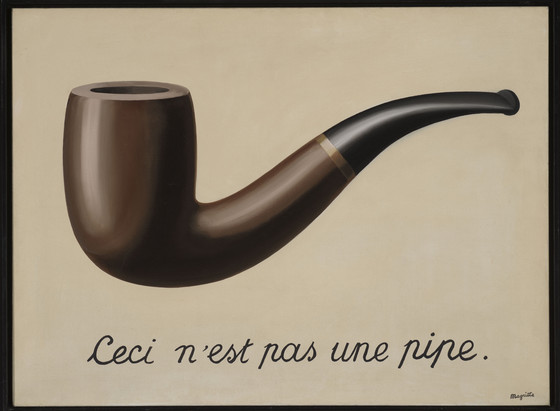
\includegraphics[width=0.7\linewidth]{images/Datenjudo/ma-150089-WEB} 

}

\caption{La trahison des images [Ceci n'est pas une pipe], René Magritte, 1929, © C. Herscovici, Brussels / Artists Rights Society (ARS), New York, http://collections.lacma.org/node/239578}\label{fig:cecie-une-pipe}
\end{figure}

Hierbei ist gemeint, einen Datensatz sozusagen auf ein Fließband zu
legen und an jedem Arbeitsplatz einen Arbeitsschritt auszuführen. Der
springende Punkt ist, dass ein Dataframe als ``Rohstoff'' eingegeben
wird und jeder Arbeitsschritt seinerseits wieder einen Datafram
ausgiebt. Damit kann man sehr schön, einen ``Flow'' an Verarbeitung
erreichen, außerdem spart man sich Tipparbeit und die Syntax wird
lesbarer. Damit das Durchpfeifen funktioniert, benötigt man Befehle, die
als Eingabe einen Dataframe erwarten und wieder einen Dataframe
zurückliefern. Das Schaubild verdeutlich beispielhaft eine Abfolge des
Durchpfeifens (s. Abb. \ref{fig:fig-durchpfeifen}).

\begin{figure}

{\centering 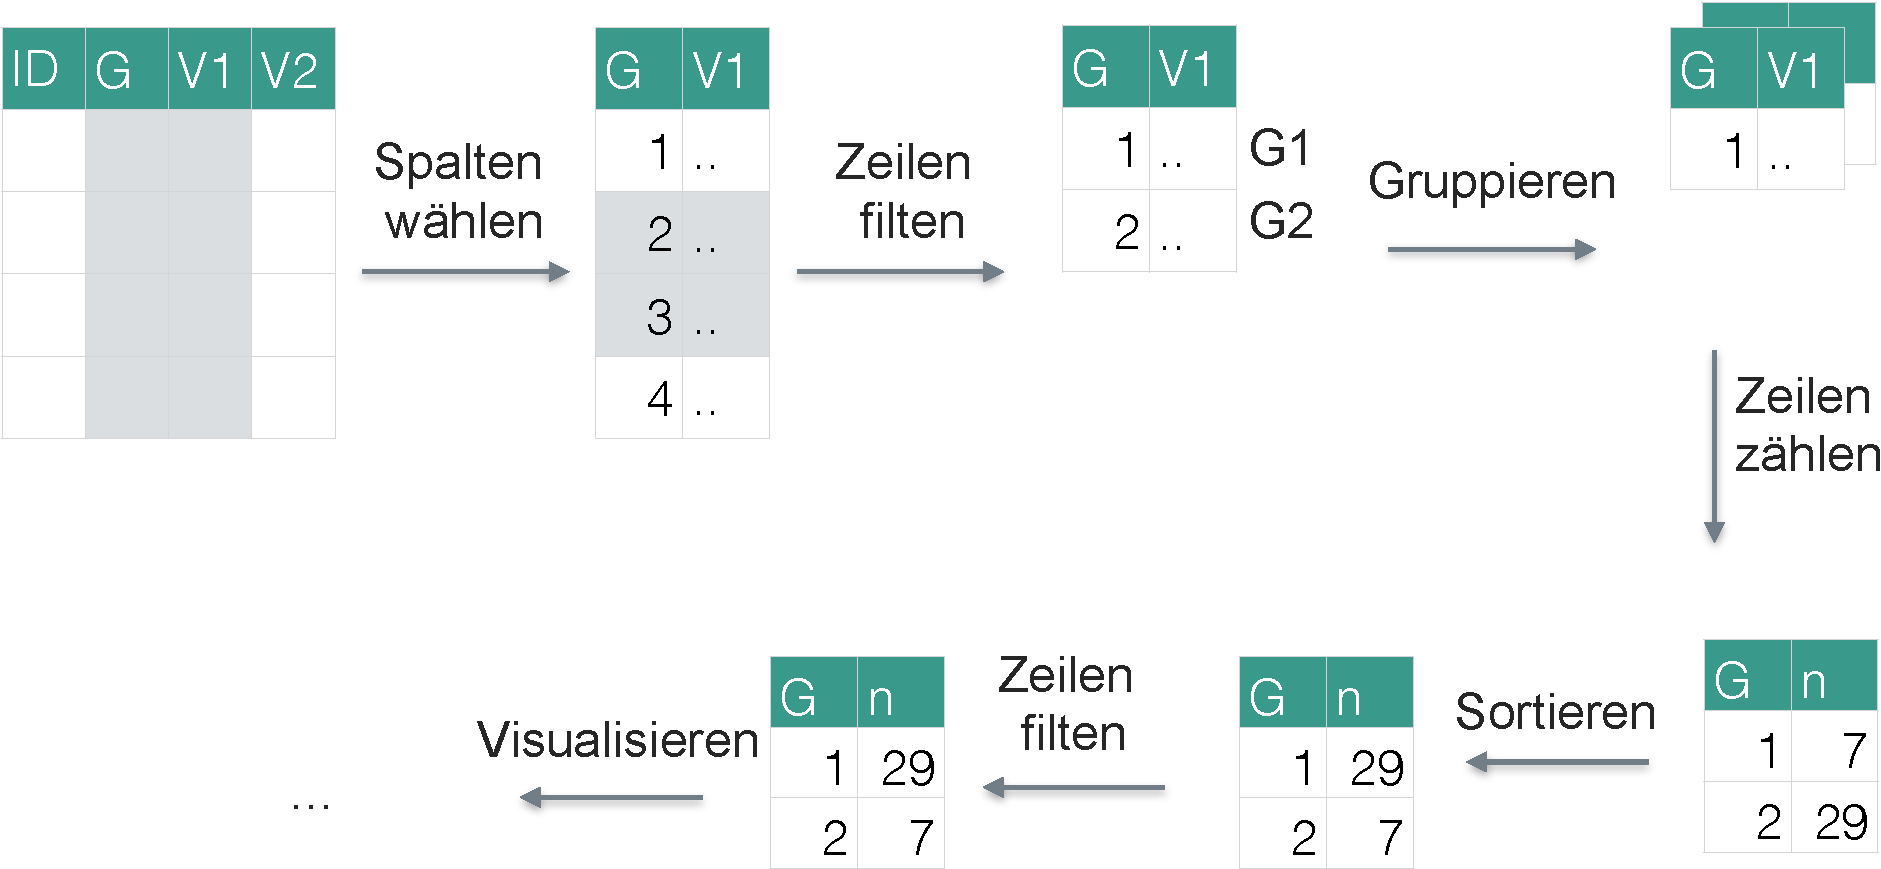
\includegraphics[width=0.8\linewidth]{images/Datenjudo/durchpfeifen} 

}

\caption{Das 'Durchpeifen'}\label{fig:fig-durchpfeifen}
\end{figure}

Die sog. ``Pfeife'' (pipe\index{Pfeife}: \texttt{\%\textgreater{}\%}) in
Anspielung an das berühmte Bild von René Magritte, verkettet Befehle
hintereinander. Das ist praktisch, da es die Syntax vereinfacht.
Vergleichen Sie mal diese Syntax

\begin{Shaded}
\begin{Highlighting}[]
\KeywordTok{filter}\NormalTok{(}\KeywordTok{summarise}\NormalTok{(}\KeywordTok{group_by}\NormalTok{(}\KeywordTok{filter}\NormalTok{(stats_test, !}\KeywordTok{is.na}\NormalTok{(score)), interest), }\DataTypeTok{mw =} \KeywordTok{mean}\NormalTok{(score)), mw >}\StringTok{ }\DecValTok{30}\NormalTok{)}
\end{Highlighting}
\end{Shaded}

mit dieser

\begin{Shaded}
\begin{Highlighting}[]
\NormalTok{stats_test %>%}\StringTok{ }
\StringTok{  }\KeywordTok{filter}\NormalTok{(!}\KeywordTok{is.na}\NormalTok{(score)) %>%}\StringTok{ }
\StringTok{  }\KeywordTok{group_by}\NormalTok{(interest) %>%}\StringTok{ }
\StringTok{  }\KeywordTok{summarise}\NormalTok{(}\DataTypeTok{mw =} \KeywordTok{mean}\NormalTok{(score)) %>%}\StringTok{ }
\StringTok{  }\KeywordTok{filter}\NormalTok{(mw >}\StringTok{ }\DecValTok{30}\NormalTok{)}
\CommentTok{#> # A tibble: 4 × 2}
\CommentTok{#>   interest    mw}
\CommentTok{#>      <int> <dbl>}
\CommentTok{#> 1        3  30.8}
\CommentTok{#> 2        5  32.5}
\CommentTok{#> 3        6  34.0}
\CommentTok{#> 4       NA  33.1}
\end{Highlighting}
\end{Shaded}

Es ist hilfreich, diese ``Pfeifen-Syntax'' in deutschen Pseudo-Code zu
übersetzen.

\BeginKnitrBlock{rmdpseudocode}
Nimm die Tabelle ``stats\_test'' UND DANN\\
filtere alle nicht-fehlenden Werte UND DANN\\
gruppiere die verbleibenden Werte nach ``interest'' UND DANN\\
bilde den Mittelwert (pro Gruppe) für ``score'' UND DANN\\
liefere nur die Werte größer als 30 zurück.
\EndKnitrBlock{rmdpseudocode}

Die zweite Syntax, in ``Pfeifenform'' ist viel einfacher zu verstehen
als die erste! Die erste Syntax ist verschachelt, man muss sie von innen
nach außen lesen. Das ist kompliziert. Die Pfeife in der 2. Syntax macht
es viel einfacher, die Snytax zu verstehen, da die Befehle
``hintereinander'' gestellt (sequenziell organisiert) sind.

Die Pfeife zerlegt die ``russische Puppe'', also ineinander
verschachelteten Code, in sequenzielle Schritte und zwar in der
richtigen Reihenfolge (entsprechend der Abarbeitung). Wir müssen den
Code nicht mehr von innen nach außen lesen (wie das bei einer
mathematischen Formel der Fall ist), sondern können wie bei einem
Kochrezept ``erstens \ldots{}, zweitens .., drittens \ldots{}'' lesen.
Die Pfeife macht die Syntax einfacher. Natürlich hätten wir die
verschachtelte Syntax in viele einzelne Befehle zerlegen können und
jeweils eine Zwischenergebnis speichern mit dem Zuweisungspfeil
\texttt{\textless{}-} und das Zwischenergebnis dann explizit an den
nächsten Befehl weitergeben. Eigentlich macht die Pfeife genau das - nur
mit weniger Tipparbeit. Und auch einfacher zu lesen. Flow!

\BeginKnitrBlock{rmdcaution}
Wenn Sie Befehle verketten mit der Pfeife, sind nur Befehle erlaubt, die
einen Datensatz als Eingabe verlangen und einen Datensatz ausgeben. Das
ist bei den hier vorgestellten Funktionen der Fall. Viele andere
Funktionen erfüllen dieses Kriterium aber nicht; in dem Fall liefert
\texttt{dplyr} eine Fehlermeldung.
\EndKnitrBlock{rmdcaution}

\subsubsection{\texorpdfstring{Spalten berechnen mit
\texttt{mutate}}{Spalten berechnen mit mutate}}\label{spalten-berechnen-mit-mutate}

Wenn man die Pfeife benutzt, ist der Befehl
\texttt{mutate}\index{dplyr::mutate} ganz praktisch: Er berechnet eine
Spalte. Normalerweise kann man einfach eine Spalte berechnen mit dem
Zuweisungsoperator:

Zum Beispiel so:

\begin{verbatim}
df$neue_spalte <- df$spalte1 + df$spalte2
\end{verbatim}

Innerhalb einer Pfeifen-Syntax geht das aber nicht (so gut). Da ist man
mit der Funtion \texttt{mutate} besser beraten; \texttt{mutate} leistest
just dasselbe wie die Pseudo-Syntax oben:

\begin{verbatim}
df %>% 
  mutate(neue_spalte = spalte1 + spalte2)
\end{verbatim}

In Worten:

\BeginKnitrBlock{rmdpseudocode}
Nimm die Tabelle ``df'' UND DANN\\
bilde eine neue Spalte mit dem Namen \texttt{neue\_spalte}, die sich
berechnet als Summe von \texttt{spalte1} und \texttt{spalte2}.
\EndKnitrBlock{rmdpseudocode}

Allerdings berücksichtigt \texttt{mutate} auch Gruppierungen. Der
Hauptvorteil ist die bessere Lesbarkeit durch Auflösen der
Verschachtelungen.

Ein konkretes Beispiel:

\begin{Shaded}
\begin{Highlighting}[]
\NormalTok{stats_test %>%}\StringTok{ }
\StringTok{  }\KeywordTok{mutate}\NormalTok{(}\DataTypeTok{bestanden =} \NormalTok{score >}\StringTok{ }\DecValTok{25}\NormalTok{) %>%}\StringTok{ }
\StringTok{  }\KeywordTok{head}\NormalTok{()}
\CommentTok{#>   X                 V_1 study_time self_eval interest score bestanden}
\CommentTok{#> 1 1 05.01.2017 13:57:01          5         8        5    29      TRUE}
\CommentTok{#> 2 2 05.01.2017 21:07:56          3         7        3    29      TRUE}
\CommentTok{#> 3 3 05.01.2017 23:33:47          5        10        6    40      TRUE}
\CommentTok{#> 4 4 06.01.2017 09:58:05          2         3        2    18     FALSE}
\CommentTok{#> 5 5 06.01.2017 14:13:08          4         8        6    34      TRUE}
\CommentTok{#> 6 6 06.01.2017 14:21:18         NA        NA       NA    39      TRUE}
\end{Highlighting}
\end{Shaded}

Diese Syntax erzeugt eine neue Spalte innerhalb von
\texttt{stats\_test}; diese Spalte prüft pro Persion, ob \texttt{score}
\textgreater{} 25 ist. Falls ja (TRUE), dann ist \texttt{bestanden}
TRUE, ansonsten ist \texttt{bestanden} FALSE (Pech). \texttt{head} zeigt
die ersten 6 Zeilen des resultierenden Dataframes an.

Abb. \ref{fig:fig-mutate} zeigt Sinnbild für \texttt{mutate}:

\begin{figure}

{\centering 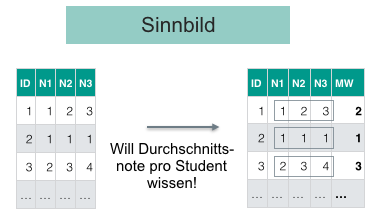
\includegraphics[width=0.7\linewidth]{images/Datenjudo/mutate} 

}

\caption{Sinnbild für mutate}\label{fig:fig-mutate}
\end{figure}

\subsubsection{Aufgaben}\label{aufgaben-6}

\begin{enumerate}
\def\labelenumi{\arabic{enumi}.}
\tightlist
\item
  Entschlüsseln Sie dieses Ungetüm! Übersetzen Sie diese Syntax auf
  Deutsch:
\end{enumerate}

\begin{Shaded}
\begin{Highlighting}[]

\KeywordTok{library}\NormalTok{(nycflights13)}
\KeywordTok{data}\NormalTok{(flights)}

\NormalTok{verspaetung <-}
\StringTok{  }\KeywordTok{filter}\NormalTok{(}
    \KeywordTok{summarise}\NormalTok{(}
    \KeywordTok{group_by}\NormalTok{(}\KeywordTok{filter}\NormalTok{(flights, !}\KeywordTok{is.na}\NormalTok{(dep_delay), month)), }\DataTypeTok{delay =} \KeywordTok{mean}\NormalTok{(dep_delay), }\DataTypeTok{n =} \KeywordTok{n}\NormalTok{()), n >}\StringTok{ }\DecValTok{10}\NormalTok{)}
 
\end{Highlighting}
\end{Shaded}

\begin{enumerate}
\def\labelenumi{\arabic{enumi}.}
\setcounter{enumi}{1}
\tightlist
\item
  Entschlüsseln Sie jetzt diese Syntax bzw. übersetzen Sie sie ins
  Deutsche:
\end{enumerate}

\begin{Shaded}
\begin{Highlighting}[]
\NormalTok{verspaetung <-}\StringTok{ }\NormalTok{flights %>%}\StringTok{ }\KeywordTok{filter}\NormalTok{(!}\KeywordTok{is.na}\NormalTok{(dep_delay)) %>%}
\KeywordTok{group_by}\NormalTok{(month) %>%}
\KeywordTok{summarise}\NormalTok{(}\DataTypeTok{delay =} \KeywordTok{mean}\NormalTok{(dep_delay), }\DataTypeTok{n =} \KeywordTok{n}\NormalTok{()) %>%}\StringTok{ }\KeywordTok{filter}\NormalTok{(n >}\StringTok{ }\DecValTok{10}\NormalTok{)}
\end{Highlighting}
\end{Shaded}

\begin{enumerate}
\def\labelenumi{\arabic{enumi}.}
\setcounter{enumi}{2}
\tightlist
\item
  (schwierig) Die Pfeife bei \texttt{arr\_delay}
\end{enumerate}

\begin{itemize}
\tightlist
\item
  Übersetzen Sie die folgende Pseudo-Syntax ins ERRRische!
\end{itemize}

\BeginKnitrBlock{rmdpseudocode}
Nehme den Datensatz \texttt{flights} UND DANN\ldots{}\\
Wähle daraus die Spalte \texttt{arr\_delay} UND DANN\ldots{}\\
Berechne den Mittelwert der Spalte UND DANN\ldots{}\\
ziehe vom Mittelwert die Spalte ab UND DANN\ldots{} quadriere die
einzelnen Differenzen UND DANN\ldots{} bilde davon den Mittelwert.
\EndKnitrBlock{rmdpseudocode}

Lösung:

\begin{Shaded}
\begin{Highlighting}[]
\NormalTok{flights %>%}\StringTok{ }
\StringTok{  }\KeywordTok{select}\NormalTok{(arr_delay) %>%}\StringTok{ }
\StringTok{  }\KeywordTok{mutate}\NormalTok{(}\DataTypeTok{arr_delay_delta =} \NormalTok{arr_delay -}\StringTok{ }\KeywordTok{mean}\NormalTok{(flights$arr_delay, }\DataTypeTok{na.rm =} \OtherTok{TRUE}\NormalTok{)) %>%}\StringTok{ }
\StringTok{  }\KeywordTok{mutate}\NormalTok{(}\DataTypeTok{arr_delay_delta_quadrat =} \NormalTok{arr_delay_delta^}\DecValTok{2}\NormalTok{) %>%}\StringTok{ }
\StringTok{  }\KeywordTok{summarise}\NormalTok{(}\DataTypeTok{arr_delay_var =} \KeywordTok{mean}\NormalTok{(arr_delay_delta_quadrat, }\DataTypeTok{na.rm =} \OtherTok{TRUE}\NormalTok{)) %>%}\StringTok{ }
\StringTok{  }\KeywordTok{summarise}\NormalTok{(}\KeywordTok{sqrt}\NormalTok{(arr_delay_var))}
\CommentTok{#> # A tibble: 1 × 1}
\CommentTok{#>   `sqrt(arr_delay_var)`}
\CommentTok{#>                   <dbl>}
\CommentTok{#> 1                  44.6}
\end{Highlighting}
\end{Shaded}

\begin{itemize}
\item
  Berechnen Sie die sd von \texttt{arr\_delay} in \texttt{flights}!
  Vergleichen Sie sie mit dem Ergebnis der vorherigen Aufgabe!\footnote{\texttt{sd(flights\$arr\_delay,\ na.rm\ =\ TRUE)}}
\item
  Was hat die Pfeifen-Syntax oben berechnet?\footnote{die sd von
    \texttt{arr\_delay}}
\end{itemize}

\subsection{Befehlsübersicht}\label{befehlsubersicht}

\begin{longtable}[]{@{}ll@{}}
\toprule
Paket::Funktion & Beschreibung\tabularnewline
\midrule
\endhead
dplyr::arrange & Sortiert Spalten\tabularnewline
dplyr::filter & Filtert Zeilen\tabularnewline
dplyr::select & Wählt Spalten\tabularnewline
dplyr::group\_by & gruppiert einen Dataframe\tabularnewline
dplyr::n & zählt Zeilen\tabularnewline
dplyr::count & zählt Zeilen nach Untergruppen\tabularnewline
\%\textgreater{}\% (dplyr) & verkettet Befehle\tabularnewline
dplyr::mutate & erzeugt/berechnet Spalten\tabularnewline
\bottomrule
\end{longtable}

\subsection{Verweise}\label{verweise}

\begin{itemize}
\item
  Die offizielle Dokumentation von \texttt{dplyr} findet sich hier:
  \url{https://cran.r-project.org/web/packages/dplyr/dplyr.pdf}.
\item
  Eine schöne Demonstration der Mächtigkeit von \texttt{dplyr} findet
  sich hier: \url{http://bit.ly/2kX9lvC}.
\item
  Die GUI ``exploratory'' ist ein ``klickbare'' Umsetzung von
  \texttt{dplyr}, mächtig, modern und sieht cool aus:
  \url{https://exploratory.io}.
\item
  \emph{R for Data Science} bietet umfangreiche Unterstützung zu diesem
  Thema (Wickham und Grolemund \protect\hyperlink{ref-r4ds}{2016}).
\end{itemize}

\section{Praxisprobleme der
Datenaufbereitung}\label{praxisprobleme-der-datenaufbereitung}

\section{Fallstudie zum Datenjudo}\label{fallstudie-zum-datenjudo}

\section{Daten visualisieren}\label{daten-visualisieren}

\section{Fallstudie zur
Visualisierung}\label{fallstudie-zur-visualisierung}

\section{Grundlagen des Modellierens}\label{mod1}

\section{Der p-Wert}\label{der-p-wert}

\section{Klassische lineare (numerische)
Regression}\label{klassische-lineare-numerische-regression}

\section{Klassifizierende Regression}\label{klassifizierende-regression}

\section{Fallstudien zum geleiteten
Modellieren}\label{fallstudien-zum-geleiteten-modellieren}

\section{nicht robust:}\label{nicht-robust}

\section{Vertiefung: Clusteranalyse}\label{vertiefung-clusteranalyse}

\section{Probeklausur}\label{probeklausur}

\section{Literaturverzeichnis}\label{literaturverzeichnis}

\hypertarget{refs}{}
\hypertarget{ref-R-rmarkdown}{}
Allaire, JJ, Joe Cheng, Yihui Xie, Jonathan McPherson, Winston Chang,
Jeff Allen, Hadley Wickham, Aron Atkins, und Rob Hyndman. 2016a.
\emph{rmarkdown: Dynamic Documents for R}.
\url{https://CRAN.R-project.org/package=rmarkdown}.

\hypertarget{ref-rmarkdown}{}
---------. 2016b. \emph{rmarkdown: Dynamic Documents for R}.
\url{https://CRAN.R-project.org/package=rmarkdown}.

\hypertarget{ref-R-gridExtra}{}
Auguie, Baptiste. 2016. \emph{gridExtra: Miscellaneous Functions for
„Grid`` Graphics}. \url{https://CRAN.R-project.org/package=gridExtra}.

\hypertarget{ref-R-BaylorEdPsych}{}
Beaujean, A. Alexander. 2012. \emph{BaylorEdPsych: R Package for Baylor
University Educational Psychology Quantitative Courses}.
\url{https://CRAN.R-project.org/package=BaylorEdPsych}.

\hypertarget{ref-R-quanteda}{}
Benoit, Kenneth, und Paul Nulty. 2016. \emph{quanteda: Quantitative
Analysis of Textual Data}.
\url{https://CRAN.R-project.org/package=quanteda}.

\hypertarget{ref-R-SnowballC}{}
Bouchet-Valat, Milan. 2014. \emph{SnowballC: Snowball stemmers based on
the C libstemmer UTF-8 library}.
\url{https://CRAN.R-project.org/package=SnowballC}.

\hypertarget{ref-breaking}{}
Briggs, William M. 2008. \emph{Breaking the Law of Averages: Real-Life
Probability and Statistics in Plain English}. Lulu.com.
\url{https://www.amazon.com/Breaking-Law-Averages-Probability-Statistics/dp/0557019907\%3FSubscriptionId\%3D0JYN1NVW651KCA56C102\%26tag\%3Dtechkie-20\%26linkCode\%3Dxm2\%26camp\%3D2025\%26creative\%3D165953\%26creativeASIN\%3D0557019907}.

\hypertarget{ref-uncertainty}{}
---------. 2016. \emph{Uncertainty: The Soul of Modeling, Probability \&
Statistics}. Springer.
\url{https://www.amazon.com/Uncertainty-Soul-Modeling-Probability-Statistics-ebook/dp/B01JEJNUJK\%3FSubscriptionId\%3D0JYN1NVW651KCA56C102\%26tag\%3Dtechkie-20\%26linkCode\%3Dxm2\%26camp\%3D2025\%26creative\%3D165953\%26creativeASIN\%3DB01JEJNUJK}.

\hypertarget{ref-bryant1995practical}{}
Bryant, PG, und MA Smith. 1995. „Practical Data Analysis: Case Studies
in Business Statistics, Homewood, IL: Richard D``. Irwin Publishing.

\hypertarget{ref-R-downloader}{}
Chang, Winston. 2015. \emph{downloader: Download Files over HTTP and
HTTPS}. \url{https://CRAN.R-project.org/package=downloader}.

\hypertarget{ref-Chapman2015}{}
Chapman, Chris, und Elea McDonnell Feit. 2015. \emph{R for Marketing
Research and Analytics}. Springer International Publishing.
doi:\href{https://doi.org/10.1007/978-3-319-14436-8}{10.1007/978-3-319-14436-8}.

\hypertarget{ref-Cleveland}{}
Cleveland, William S. 1993. \emph{Visualizing Data}. Hobart Press.
\url{https://www.amazon.com/Visualizing-Data-William-S-Cleveland/dp/0963488406\%3FSubscriptionId\%3D0JYN1NVW651KCA56C102\%26tag\%3Dtechkie-20\%26linkCode\%3Dxm2\%26camp\%3D2025\%26creative\%3D165953\%26creativeASIN\%3D0963488406}.

\hypertarget{ref-cobb2007introductory}{}
Cobb, George W. 2007. „The introductory statistics course: a Ptolemaic
curriculum?`` \emph{Technology Innovations in Statistics Education} 1
(1).

\hypertarget{ref-cortez2009modeling}{}
Cortez, Paulo, António Cerdeira, Fernando Almeida, Telmo Matos, und José
Reis. 2009. „Modeling wine preferences by data mining from
physicochemical properties``. \emph{Decision Support Systems} 47 (4).
Elsevier: 547--53.

\hypertarget{ref-R-ggdendro}{}
de Vries, Andrie, und Brian D. Ripley. 2016. \emph{ggdendro: Create
Dendrograms and Tree Diagrams Using 'ggplot2'}.
\url{https://CRAN.R-project.org/package=ggdendro}.

\hypertarget{ref-R-tm}{}
Feinerer, Ingo, und Kurt Hornik. 2015. \emph{tm: Text Mining Package}.
\url{https://CRAN.R-project.org/package=tm}.

\hypertarget{ref-R-wordcloud}{}
Fellows, Ian. 2014. \emph{wordcloud: Word Clouds}.
\url{https://CRAN.R-project.org/package=wordcloud}.

\hypertarget{ref-R-car}{}
Fox, John, und Sanford Weisberg. 2016. \emph{car: Companion to Applied
Regression}. \url{https://CRAN.R-project.org/package=car}.

\hypertarget{ref-gigerenzer1980}{}
Gigerenzer, Gerd. 1980. \emph{Messung und Modellbildung in der
Psychologie (Uni-Taschenbucher. Psychologie, Padagogik, Soziologie,
Psychiatrie) (German Edition)}. E. Reinhardt.
\url{https://www.amazon.com/Modellbildung-Psychologie-Uni-Taschenbucher-Soziologie-Psychiatrie/dp/3497008958\%3FSubscriptionId\%3D0JYN1NVW651KCA56C102\%26tag\%3Dtechkie-20\%26linkCode\%3Dxm2\%26camp\%3D2025\%26creative\%3D165953\%26creativeASIN\%3D3497008958}.

\hypertarget{ref-Gigerenzer2004}{}
---------. 2004. „Mindless statistics``. \emph{The Journal of
Socio-Economics} 33 (5). Elsevier BV: 587--606.
doi:\href{https://doi.org/10.1016/j.socec.2004.09.033}{10.1016/j.socec.2004.09.033}.

\hypertarget{ref-grolemund2014cognitive}{}
Grolemund, Garrett, und Hadley Wickham. 2014. „A cognitive
interpretation of data analysis``. \emph{International Statistical
Review} 82 (2). Wiley Online Library: 184--204.

\hypertarget{ref-R-arules}{}
Hahsler, Michael, Christian Buchta, Bettina Gruen, und Kurt Hornik.
2016. \emph{arules: Mining Association Rules and Frequent Itemsets}.
\url{https://CRAN.R-project.org/package=arules}.

\hypertarget{ref-R-arulesViz}{}
Hahsler, Michael, und Sudheer Chelluboina. 2016. \emph{arulesViz:
Visualizing Association Rules and Frequent Itemsets}.
\url{https://CRAN.R-project.org/package=arulesViz}.

\hypertarget{ref-hamermesh2005beauty}{}
Hamermesh, Daniel S, und Amy Parker. 2005. „Beauty in the classroom:
Instructors' pulchritude and putative pedagogical productivity``.
\emph{Economics of Education Review} 24 (4). Elsevier: 369--76.

\hypertarget{ref-hardin2015data}{}
Hardin, Johanna, Roger Hoerl, Nicholas J Horton, Deborah Nolan, Ben
Baumer, Olaf Hall-Holt, Paul Murrell, u.~a. 2015. „Data science in
statistics curricula: Preparing students to ‚Think with Data```.
\emph{The American Statistician} 69 (4). Taylor \& Francis: 343--53.

\hypertarget{ref-Head2015}{}
Head, Megan L., Luke Holman, Rob Lanfear, Andrew T. Kahn, und Michael D.
Jennions. 2015. „The Extent and Consequences of P-Hacking in Science``.
\emph{PLOS Biology} 13 (3). Public Library of Science (PLoS): e1002106.
doi:\href{https://doi.org/10.1371/journal.pbio.1002106}{10.1371/journal.pbio.1002106}.

\hypertarget{ref-R-titanic}{}
Hendricks, Paul. 2015. \emph{titanic: Titanic Passenger Survival Data
Set}. \url{https://CRAN.R-project.org/package=titanic}.

\hypertarget{ref-tm}{}
Ingo Feinerer, Kurt Hornik, und David Meyer. 2008. „Text Mining
Infrastructure in R``. \emph{Journal of Statistical Software} 25 (5):
1--54. \url{http://www.jstatsoft.org/v25/i05/}.

\hypertarget{ref-R-corrr}{}
Jackson, Simon. 2016. \emph{corrr: Correlations in R}.
\url{https://CRAN.R-project.org/package=corrr}.

\hypertarget{ref-R-ISLR}{}
James, Gareth, Daniela Witten, Trevor Hastie, und Rob Tibshirani. 2013a.
\emph{ISLR: Data for An Introduction to Statistical Learning with
Applications in R}. \url{https://CRAN.R-project.org/package=ISLR}.

\hypertarget{ref-introstatlearning}{}
James, Gareth, Daniela Witten, Trevor Hastie, und Robert Tibshirani.
2013b. \emph{An introduction to statistical learning}. Bd. 6. Springer.

\hypertarget{ref-james2013introduction}{}
---------. 2013c. \emph{An introduction to statistical learning}. Bd. 6.
Springer.

\hypertarget{ref-tidytextminig}{}
Julia, PhD Silge, und PhD Robinson David. 2017. \emph{Text Mining with
R: A tidy approach}. O'Reilly Media.
\url{https://www.amazon.com/Text-Mining-R-tidy-approach/dp/1491981652\%3FSubscriptionId\%3D0JYN1NVW651KCA56C102\%26tag\%3Dtechkie-20\%26linkCode\%3Dxm2\%26camp\%3D2025\%26creative\%3D165953\%26creativeASIN\%3D1491981652}.

\hypertarget{ref-kim2015okcupid}{}
Kim, Albert Y, und Adriana Escobedo-Land. 2015. „OkCupid Data for
Introductory Statistics and Data Science Courses``. \emph{Journal of
Statistics Education} 23 (2). Citeseer: n2.

\hypertarget{ref-R-okcupiddata}{}
Kim, Albert Y., und Adriana Escobedo-Land. 2016. \emph{okcupiddata:
OkCupid Profile Data for Introductory Statistics and Data Science
Courses}. \url{https://CRAN.R-project.org/package=okcupiddata}.

\hypertarget{ref-kraemer2011wir}{}
Krämer, W. 2011. \emph{Wie wir uns von falschen Theorien täuschen
lassen}. Berlin University Press.
\url{https://books.google.de/books?id=HWUKaAEACAAJ}.

\hypertarget{ref-kuhn2013applied}{}
Kuhn, Max, und Kjell Johnson. 2013. \emph{Applied predictive modeling}.
Bd. 26. Springer.

\hypertarget{ref-R-scatterplot3d}{}
Ligges, Uwe, Martin Maechler, und Sarah Schnackenberg. 2017.
\emph{scatterplot3d: 3D Scatter Plot}.
\url{https://CRAN.R-project.org/package=scatterplot3d}.

\hypertarget{ref-R-rpart.plot}{}
Milborrow, Stephen. 2017. \emph{rpart.plot: Plot 'rpart' Models: An
Enhanced Version of 'plot.rpart'}.
\url{https://CRAN.R-project.org/package=rpart.plot}.

\hypertarget{ref-moore1990uncertainty}{}
Moore, David S. 1990. „Uncertainty``. \emph{On the shoulders of giants:
New approaches to numeracy}. ERIC, 95--137.

\hypertarget{ref-R-tokenizers}{}
Mullen, Lincoln. 2016. \emph{tokenizers: A Consistent Interface to
Tokenize Natural Language Text}.
\url{https://CRAN.R-project.org/package=tokenizers}.

\hypertarget{ref-R-RColorBrewer}{}
Neuwirth, Erich. 2014. \emph{RColorBrewer: ColorBrewer Palettes}.
\url{https://CRAN.R-project.org/package=RColorBrewer}.

\hypertarget{ref-R-pdftools}{}
Ooms, Jeroen. 2016. \emph{pdftools: Text Extraction and Rendering of PDF
Documents}. \url{https://CRAN.R-project.org/package=pdftools}.

\hypertarget{ref-peirce1955abduction}{}
Peirce, Charles S. 1955. „Abduction and induction``. \emph{Philosophical
writings of Peirce} 11. New York.

\hypertarget{ref-peng2015art}{}
Peng, Roger D, und Elizabeth Matsui. 2015. „The Art of Data Science``.
\emph{A Guide for Anyone Who Works with Data. Skybrude Consulting} 200:
162.

\hypertarget{ref-R-nFactors}{}
Raiche, Gilles, und David Magis. 2011. \emph{nFactors: Parallel Analysis
and Non Graphical Solutions to the Cattell Scree Test}.
\url{https://CRAN.R-project.org/package=nFactors}.

\hypertarget{ref-R-wesanderson}{}
Ram, Karthik, und Hadley Wickham. 2015. \emph{wesanderson: A Wes
Anderson Palette Generator}.
\url{https://CRAN.R-project.org/package=wesanderson}.

\hypertarget{ref-R-compute.es}{}
Re, AC Del. 2014. \emph{compute.es: Compute Effect Sizes}.
\url{https://CRAN.R-project.org/package=compute.es}.

\hypertarget{ref-remquahey2010}{}
Remus, R., U. Quasthoff, und G. Heyer. 2010. „SentiWS -- a Publicly
Available German-language Resource for Sentiment Analysis``. In
\emph{Proceedings of the 7th International Language Resources and
Evaluation (LREC'10)}, 1168--71.

\hypertarget{ref-R-MASS}{}
Ripley, Brian. 2016. \emph{MASS: Support Functions and Datasets for
Venables and Ripley's MASS}.
\url{https://CRAN.R-project.org/package=MASS}.

\hypertarget{ref-nycflights13}{}
RITA, Bureau of transportation statistics. 2013. „nycflights13``.
\href{http://www.transtats.bts.gov/DL\%7B/_\%7DSelectFields.asp?Table\%7B/_\%7DID=236}{http://www.transtats.bts.gov/DL\{\textbackslash{}\_\}SelectFields.asp?Table\{\textbackslash{}\_\}ID=236}.

\hypertarget{ref-R-gutenbergr}{}
Robinson, David. 2016. \emph{gutenbergr: Download and Process Public
Domain Works from Project Gutenberg}.
\url{https://cran.rstudio.com/package=gutenbergr}.

\hypertarget{ref-R-broom}{}
Robinson, David, Matthieu Gomez, Boris Demeshev, Dieter Menne, Benjamin
Nutter, Luke Johnston, Ben Bolker, Francois Briatte, und Hadley Wickham.
2015. \emph{broom: Convert Statistical Analysis Objects into Tidy Data
Frames}. \url{https://CRAN.R-project.org/package=broom}.

\hypertarget{ref-R-tidytext}{}
Robinson, David, und Julia Silge. 2016. \emph{tidytext: Text Mining
using 'dplyr', 'ggplot2', and Other Tidy Tools}.
\url{https://CRAN.R-project.org/package=tidytext}.

\hypertarget{ref-sep-statistics}{}
Romeijn, Jan-Willem. 2016. „Philosophy of Statistics``. In \emph{The
Stanford Encyclopedia of Philosophy}, herausgegeben von Edward N. Zalta,
Winter 2016.
\url{http://plato.stanford.edu/archives/win2016/entries/statistics/}.

\hypertarget{ref-ruckerinfinity}{}
Rucker, R. o.~J. \emph{Infinity and the Mind}. ????? ???????
\url{https://books.google.de/books?id=MD0UAwAAQBAJ}.

\hypertarget{ref-Sauer_2016}{}
Sauer, Sebastian. 2016. „Extraversion Dataset``. Open Science Framework.
doi:\href{https://doi.org/10.17605/OSF.IO/4KGZH}{10.17605/OSF.IO/4KGZH}.

\hypertarget{ref-Sauer_2017}{}
---------. 2017a. „Dataset ‚predictors of performance in stats test```.
Open Science Framework.
doi:\href{https://doi.org/10.17605/OSF.IO/SJHUY}{10.17605/OSF.IO/SJHUY}.

\hypertarget{ref-Sauer_2017a}{}
---------. 2017b. „Dataset ‚Height and shoe size```. Open Science
Framework.
doi:\href{https://doi.org/10.17605/OSF.IO/JA9DW}{10.17605/OSF.IO/JA9DW}.

\hypertarget{ref-sauer_wolff}{}
Sauer, Sebastian, und Alexander Wolff. 2016. „The effect of a status
symbol on success in online dating: an experimental study (data
paper)``. \emph{The Winnower}, August.
doi:\href{https://doi.org/10.15200/winn.147241.13309}{10.15200/winn.147241.13309}.

\hypertarget{ref-R-GGally}{}
Schloerke, Barret, Jason Crowley, Di Cook, Francois Briatte, Moritz
Marbach, Edwin Thoen, Amos Elberg, und Joseph Larmarange. 2016.
\emph{GGally: Extension to 'ggplot2'}.
\url{https://CRAN.R-project.org/package=GGally}.

\hypertarget{ref-R-janeaustenr}{}
Silge, Julia. 2016. \emph{janeaustenr: Jane Austen's Complete Novels}.
\url{https://CRAN.R-project.org/package=janeaustenr}.

\hypertarget{ref-tidytext-archive}{}
Silge, Julia, David Robinson, und Jim Hester. 2016. „tidytext: Text
mining using dplyr, ggplot2, and other tidy tools``.
doi:\href{https://doi.org/10.5281/zenodo.56714}{10.5281/zenodo.56714}.

\hypertarget{ref-Silge2016}{}
Silge, Julia, und David Robinson. 2016. „tidytext: Text Mining and
Analysis Using Tidy Data Principles in R``. \emph{The Journal of Open
Source Software} 1 (3). The Open Journal.
doi:\href{https://doi.org/10.21105/joss.00037}{10.21105/joss.00037}.

\hypertarget{ref-suppes1962basic}{}
Suppes, Patrick, und Joseph L Zinnes. 1962. \emph{Basic measurement
theory}. Institute for mathematical studies in the social sciences.

\hypertarget{ref-oxford}{}
\emph{The Oxford Dictionary of Statistical Terms}. 2006. Oxford
University Press.
\url{https://www.amazon.com/Oxford-Dictionary-Statistical-Terms/dp/0199206139\%3FSubscriptionId\%3D0JYN1NVW651KCA56C102\%26tag\%3Dtechkie-20\%26linkCode\%3Dxm2\%26camp\%3D2025\%26creative\%3D165953\%26creativeASIN\%3D0199206139}.

\hypertarget{ref-R-rpart}{}
Therneau, Terry, Beth Atkinson, und Brian Ripley. 2015. \emph{rpart:
Recursive Partitioning and Regression Trees}.
\url{https://CRAN.R-project.org/package=rpart}.

\hypertarget{ref-1930824149}{}
Tufte, Edward R. 1990. \emph{Envisioning Information}. Graphics Press.
\url{https://www.amazon.com/Envisioning-Information-Edward-R-Tufte/dp/1930824149\%3FSubscriptionId\%3D0JYN1NVW651KCA56C102\%26tag\%3Dtechkie-20\%26linkCode\%3Dxm2\%26camp\%3D2025\%26creative\%3D165953\%26creativeASIN\%3D1930824149}.

\hypertarget{ref-1930824130}{}
---------. 2001. \emph{The Visual Display of Quantitative Information}.
Graphics Press.
\url{https://www.amazon.com/Visual-Display-Quantitative-Information/dp/1930824130\%3FSubscriptionId\%3D0JYN1NVW651KCA56C102\%26tag\%3Dtechkie-20\%26linkCode\%3Dxm2\%26camp\%3D2025\%26creative\%3D165953\%26creativeASIN\%3D1930824130}.

\hypertarget{ref-1930824165}{}
---------. 2006. \emph{Beautiful Evidence}. Graphics Press.
\url{https://www.amazon.com/Beautiful-Evidence-Edward-R-Tufte/dp/1930824165\%3FSubscriptionId\%3D0JYN1NVW651KCA56C102\%26tag\%3Dtechkie-20\%26linkCode\%3Dxm2\%26camp\%3D2025\%26creative\%3D165953\%26creativeASIN\%3D1930824165}.

\hypertarget{ref-R-SDMTools}{}
VanDerWal, Jeremy, Lorena Falconi, Stephanie Januchowski, Luke Shoo, und
Collin Storlie. 2014. \emph{SDMTools: Species Distribution Modelling
Tools: Tools for processing data associated with species distribution
modelling exercises}. \url{https://CRAN.R-project.org/package=SDMTools}.

\hypertarget{ref-Wagenmakers2007}{}
Wagenmakers, Eric-Jan. 2007. „A practical solution to the pervasive
problems ofp values``. \emph{Psychonomic Bulletin \& Review} 14 (5).
Springer Nature: 779--804.
doi:\href{https://doi.org/10.3758/bf03194105}{10.3758/bf03194105}.

\hypertarget{ref-R-gplots}{}
Warnes, Gregory R., Ben Bolker, Lodewijk Bonebakker, Robert Gentleman,
Wolfgang Huber Andy Liaw, Thomas Lumley, Martin Maechler, u.~a. 2016.
\emph{gplots: Various R Programming Tools for Plotting Data}.
\url{https://CRAN.R-project.org/package=gplots}.

\hypertarget{ref-R-corrplot}{}
Wei, Taiyun, und Viliam Simko. 2016. \emph{corrplot: Visualization of a
Correlation Matrix}. \url{https://CRAN.R-project.org/package=corrplot}.

\hypertarget{ref-Wicherts2016}{}
Wicherts, Jelte M., Coosje L. S. Veldkamp, Hilde E. M. Augusteijn,
Marjan Bakker, Robbie C. M. van Aert, und Marcel A. L. M. van Assen.
2016. „Degrees of Freedom in Planning, Running, Analyzing, and Reporting
Psychological Studies: A Checklist to Avoid p-Hacking``. \emph{Frontiers
in Psychology} 7 (November). Frontiers Media SA.
doi:\href{https://doi.org/10.3389/fpsyg.2016.01832}{10.3389/fpsyg.2016.01832}.

\hypertarget{ref-R-ggplot2}{}
Wickham, Hadley. 2009. \emph{ggplot2: Elegant Graphics for Data
Analysis}. Springer-Verlag New York. \url{http://ggplot2.org}.

\hypertarget{ref-tidydata}{}
---------. 2014. „Tidy Data``. \emph{Journal of Statistical Software} 59
(1): 1--23.
doi:\href{https://doi.org/10.18637/jss.v059.i10}{10.18637/jss.v059.i10}.

\hypertarget{ref-R-reshape2}{}
---------. 2016a. \emph{reshape2: Flexibly Reshape Data: A Reboot of the
Reshape Package}. \url{https://CRAN.R-project.org/package=reshape2}.

\hypertarget{ref-R-tidyr}{}
---------. 2016b. \emph{tidyr: Easily Tidy Data with `spread()` and
`gather()` Functions}. \url{https://CRAN.R-project.org/package=tidyr}.

\hypertarget{ref-R-nycflights13}{}
---------. 2017a. \emph{nycflights13: Flights that Departed NYC in
2013}. \url{https://CRAN.R-project.org/package=nycflights13}.

\hypertarget{ref-R-stringr}{}
---------. 2017b. \emph{stringr: Simple, Consistent Wrappers for Common
String Operations}. \url{https://CRAN.R-project.org/package=stringr}.

\hypertarget{ref-R-tidyverse}{}
---------. 2017c. \emph{tidyverse: Easily Install and Load 'Tidyverse'
Packages}. \url{https://CRAN.R-project.org/package=tidyverse}.

\hypertarget{ref-R-readr}{}
Wickham, Hadley, Jim Hester, und Romain Francois. 2016a. \emph{readr:
Read Tabular Data}. \url{https://CRAN.R-project.org/package=readr}.

\hypertarget{ref-readr}{}
---------. 2016b. \emph{readr: Read Tabular Data}.
\url{https://CRAN.R-project.org/package=readr}.

\hypertarget{ref-R-dplyr}{}
Wickham, Hadley, und Romain Francois. 2016. \emph{dplyr: A Grammar of
Data Manipulation}. \url{https://CRAN.R-project.org/package=dplyr}.

\hypertarget{ref-r4ds}{}
Wickham, Hadley, und Garrett Grolemund. 2016. \emph{R for Data Science:
Visualize, Model, Transform, Tidy, and Import Data}. O'Reilly Media.
\url{https://www.amazon.com/Data-Science-Visualize-Model-Transform/dp/1491910399\%3FSubscriptionId\%3D0JYN1NVW651KCA56C102\%26tag\%3Dtechkie-20\%26linkCode\%3Dxm2\%26camp\%3D2025\%26creative\%3D165953\%26creativeASIN\%3D1491910399}.

\hypertarget{ref-wild1999statistical}{}
Wild, Chris J, und Maxine Pfannkuch. 1999. „Statistical thinking in
empirical enquiry``. \emph{International Statistical Review} 67 (3).
Wiley Online Library: 223--48.

\hypertarget{ref-R-lsa}{}
Wild, Fridolin. 2015. \emph{lsa: Latent Semantic Analysis}.
\url{https://CRAN.R-project.org/package=lsa}.

\hypertarget{ref-wilkinson2006grammar}{}
Wilkinson, Leland. 2006. \emph{The grammar of graphics}. Springer
Science \& Business Media.

\hypertarget{ref-xie2015}{}
Xie, Yihui. 2015. \emph{Dynamic Documents with R and knitr}. 2nd Aufl.
Boca Raton, Florida: Chapman; Hall/CRC. \url{http://yihui.name/knitr/}.

\hypertarget{ref-R-knitr}{}
---------. 2016. \emph{knitr: A General-Purpose Package for Dynamic
Report Generation in R}. \url{https://CRAN.R-project.org/package=knitr}.

\hypertarget{ref-zumel2014practical}{}
Zumel, Nina, John Mount, und Jim Porzak. 2014. \emph{Practical data
science with R}. Manning.

\printindex


\end{document}
